\documentclass[t,compress,mathserif,12pt,xcolor=dvipsnames]{beamer}
\setbeamertemplate{bibliography item}{\insertbiblabel}
\usepackage{etex}
\reserveinserts{28}
\definecolor{bleuUni}{RGB}{3, 184, 222}
\definecolor{marronUni}{RGB}{68, 58, 49}
\usecolortheme[named=bleuUni]{structure}
\usepackage[bars]{beamerthemetree} % Beamer theme v 2.2
\usepackage{multimedia}
\usepackage[utf8]{inputenc}
%\usepackage[frenchb]{babel}
\usepackage[T1]{fontenc}
\usepackage{kmath,kerkis}
\usepackage{xmpmulti}
%\usepackage{mathpazo}
%\usepackage[bitstream-charter]{mathdesign}
%\usepackage{lmodern}
\usepackage{booktabs}
\usepackage{multirow}
\usepackage{pgfplots}
\pgfplotsset{compat=newest}
\usepackage{tikz}
\usetikzlibrary{patterns, shapes, arrows}
\usepackage{mathtools}
\usepackage{listings}
\usepackage{eulervm}
\usepackage{pifont}% http://ctan.org/pkg/pifont
\newcommand{\cmark}{\ding{51}}%
\newcommand{\xmark}{\ding{55}}%
\usepackage{listings}
\usepackage{array}
\newcolumntype{L}[1]{>{\raggedright\let\newline\\\arraybackslash\hspace{0pt}}m{#1}}
\newcolumntype{C}[1]{>{\centering\let\newline\\\arraybackslash\hspace{0pt}}m{#1}}
\newcolumntype{R}[1]{>{\raggedleft\let\newline\\\arraybackslash\hspace{0pt}}m{#1}}

\lstset{
  language=C++,
  basicstyle=\tiny\ttfamily,
  numbers=left,
  numberstyle=\tiny\ttfamily,
  stepnumber=1,
  numbersep=5pt,
  backgroundcolor=\color{white},
  showspaces=false,
  showstringspaces=false,
  showtabs=false,
  frame=single,
  tabsize=2,
  captionpos=b,
  breaklines=true,
  breakatwhitespace=false,
  escapeinside={(*@}{@*)},
  identifierstyle=\ttfamily,
  keywordstyle=\color[rgb]{0,0,1},
  commentstyle=\color[rgb]{0.133,0.545,0.133},
  stringstyle=\color[rgb]{0.627,0.126,0.941},
  moredelim=[is][\underbar]{**}{**},
}

\lstdefinestyle{mycpp}
{
    language = C++,
    % numbers=left,
    % numbersep=0.3em,
    escapeinside={(*@}{@*)},
    tabsize=2,
    % basicstyle=\tiny\ttfamily,
    morekeywords = {constexpr,int8_t,int16_t,int32_t, size_t},
    % commentstyle=\color{comment-color},
}

\usepackage[backend=biber, style=ieee]{biblatex}
\addbibresource{bibli.bib}
\renewcommand\mkbibacro[1]{{\footnotesize\MakeUppercase{#1}}}

\mode<presentation>
\newcommand*\oldmacro{}%
\let\oldmacro\insertshorttitle%
\renewcommand*\insertshorttitle{%
 \oldmacro\hfill%
\insertframenumber\,/\,\inserttotalframenumber}
\setbeamertemplate{footline}[frame number]
\setbeamersize{text margin left=10pt,text margin right=10pt}
\setbeamerfont{frametitle}{size=\large}
\setbeamertemplate{frametitle}{ \nointerlineskip \begin{beamercolorbox}[wd=\paperwidth,ht=2.2ex,dp=0.5ex,left]{frametitle} \hspace*{3.1ex}\strut\bfseries\color{bleuUni!15!white}\insertframetitle\strut\par \end{beamercolorbox}}

\setbeamertemplate{bibliography item}{\insertbiblabel}
  \definecolor{bluecite}{HTML}{009DE0}


\makeatletter
\def\beamer@andinst{\\[0.1em]}
\makeatother
%~~~~~~~~~~~~~~~~~~~~~~~~~~~~~~~~~~~~~~~~~~~~~~~~~~~~~~~~~~~
%\setbeamercovered{higly dynamic}
\usetheme{Ilmenau} % Beamer theme v 3.0
%\useoutertheme[subsection=true]{smoothbars}%Beamer Outer Theme-circles on top
\setbeamercolor{section in head/foot}{bg=marronUni}

\useinnertheme{circles} %rectangle bullet points instead of circle ones
\usepackage{beamerthemebars}
\setbeamercolor{navigation symbols dimmed}{fg=red!80!black}
\setbeamercolor{navigation symbols}{fg=red!80!black}
\setbeamertemplate{navigation symbols}{}%remove navigation symbols
%~~~~~~~~~~~~~~~~~~~~~~~~~~~~~~~~~~~~~~~~~~~~~~~~~~~~~~~~~~~~~~~~~~~~~
\title{\textbf{Candidature au poste de \\ Maître de conférence en électronique numérique}}
%\subtitle{algorithms et arhitecture}\hspace{10.7cm}
\author[Mathieu Léonardon\hspace{3.01cm}\url{https://mathieuleonardon.com}\hspace{1.0cm}{mathieu.leonardon@ims-bordeaux.fr}]{\Large{Mathieu Léonardon}\vspace{-0.5cm}}
\titlegraphic{
\includegraphics[height=1.5cm]{fig/labsticc.png}\quad
\includegraphics[height=2cm]{logos/IMT_Atlantique_logo.png}}
\date{22 Novembre 2019}
\input{colors}

\definecolor{dgreen}{rgb}{0.,0.6,0.}
\definecolor{milano}{rgb}{0.458824, 0.050980, 0.058824}
\definecolor{bahama}{rgb}{0.066667, 0.298039, 0.443137}
\definecolor{blupres}{RGB}{0, 157, 224}
\definecolor{redpres}{RGB}{204, 0, 0}

\newcommand\blfootnote[1]{%
  \begingroup
  \renewcommand\thefootnote{}\footnote{#1}%
  \addtocounter{footnote}{-1}%
  \endgroup
}



\newcommand{\RED} [1]{\textcolor{Paired-5}{\textbf{#1}}}
\newcommand{\ORANGE} [1]{\textcolor{orange}{\textbf{#1}}}
\newcommand{\GREEN} [1]{\textcolor{Paired-3}{\textbf{#1}}}
\newcommand{\BLUE} [1]{\textcolor{bleuUni}{\textbf{#1}}}

\newcommand{\MILANO} [1]{\textcolor{milano}{#1}}
\newcommand{\BAHAMA} [1]{\textcolor{bahama}{#1}}

\usepackage{textpos}
%\usepackage{stmaryrd}
\usepackage{amsbsy}
\usepackage{makecell}
%\usepackage{fourier-orns}
% \usepackage{tikz}
% \usetikzlibrary{patterns, shapes, arrows, shapes.multipart}

\usepackage{etoolbox}
\AtBeginSection[]
{
	% \ifnumcomp{\value{section}}{=}{1}{}{
\begin{frame}[t]{Plan}
\centering
\tableofcontents[
  currentsection,
  currentsubsection,
  sectionstyle=show/show,
  subsectionstyle=show/show/shaded,
]
\end{frame}
% }
}
% \AtBeginSubsection[]
% {
% 	\begin{frame}[t]{}
% \tableofcontents[
% currentsection,
% sectionstyle=show/show,
% subsectionstyle=show/shaded/hide
% ]
% 	\end{frame}
% }


% \defbeamertemplate*{title page}{customized}[1][]
% {
%   \usebeamerfont{title}\inserttitle\par
%   \usebeamerfont{subtitle}\usebeamercolor[fg]{subtitle}\insertsubtitle\par
%   \bigskip
%   \usebeamerfont{author}\insertauthor\par
%   \usebeamerfont{institute}\insertinstitute\par
%   \usebeamerfont{date}\insertdate\par
%   \usebeamercolor[fg]{titlegraphic}\inserttitlegraphic
% }

\bibliography{bibli}


% \includeonly{part2}

\begin{document}

\begin{frame}[t]
\titlepage
\end{frame}

\section{Cursus}
\subsection{Formation d'ingénieur}
\begin{frame}[t]{Formation d'ingénieur - Cours}
  \begin{minipage}[t][5.0cm][t]{\textwidth}
    \begin{columns}[T]
      \begin{column}{0.63\textwidth}
        \begin{itemize}
          \item<+-> ENSEIRB-Matmeca (Bordeaux)
          \item<+-> "Systèmes Electroniques Embarqués"
          \begin{itemize}
            \item<+-> FPGA et ASIC (Langage VHDL)
            \item<+-> Architecture des ordinateurs
            \item<+-> Programmation uC
            \item<+-> OS embarqués
          \end{itemize}
        \end{itemize}
      \end{column}
      \begin{column}{0.04\textwidth}

      \end{column}
      \begin{column}{0.33\textwidth}
        \only<1->{\centering
\includegraphics[width=0.5\textwidth]{fig/UBx}\\ \vspace{0.5cm}}
        \only<3->{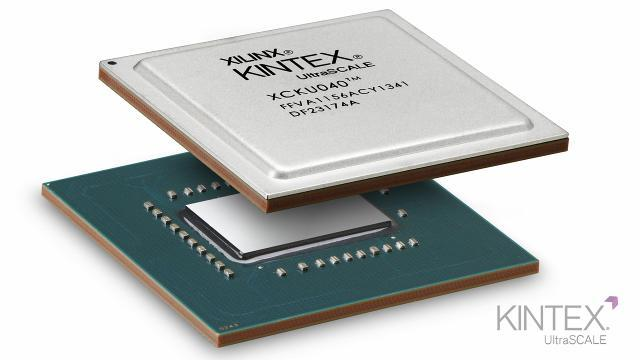
\includegraphics[width=0.5\textwidth]{fig/fpga}\\ \vspace{0.5cm}}
        \only<4->{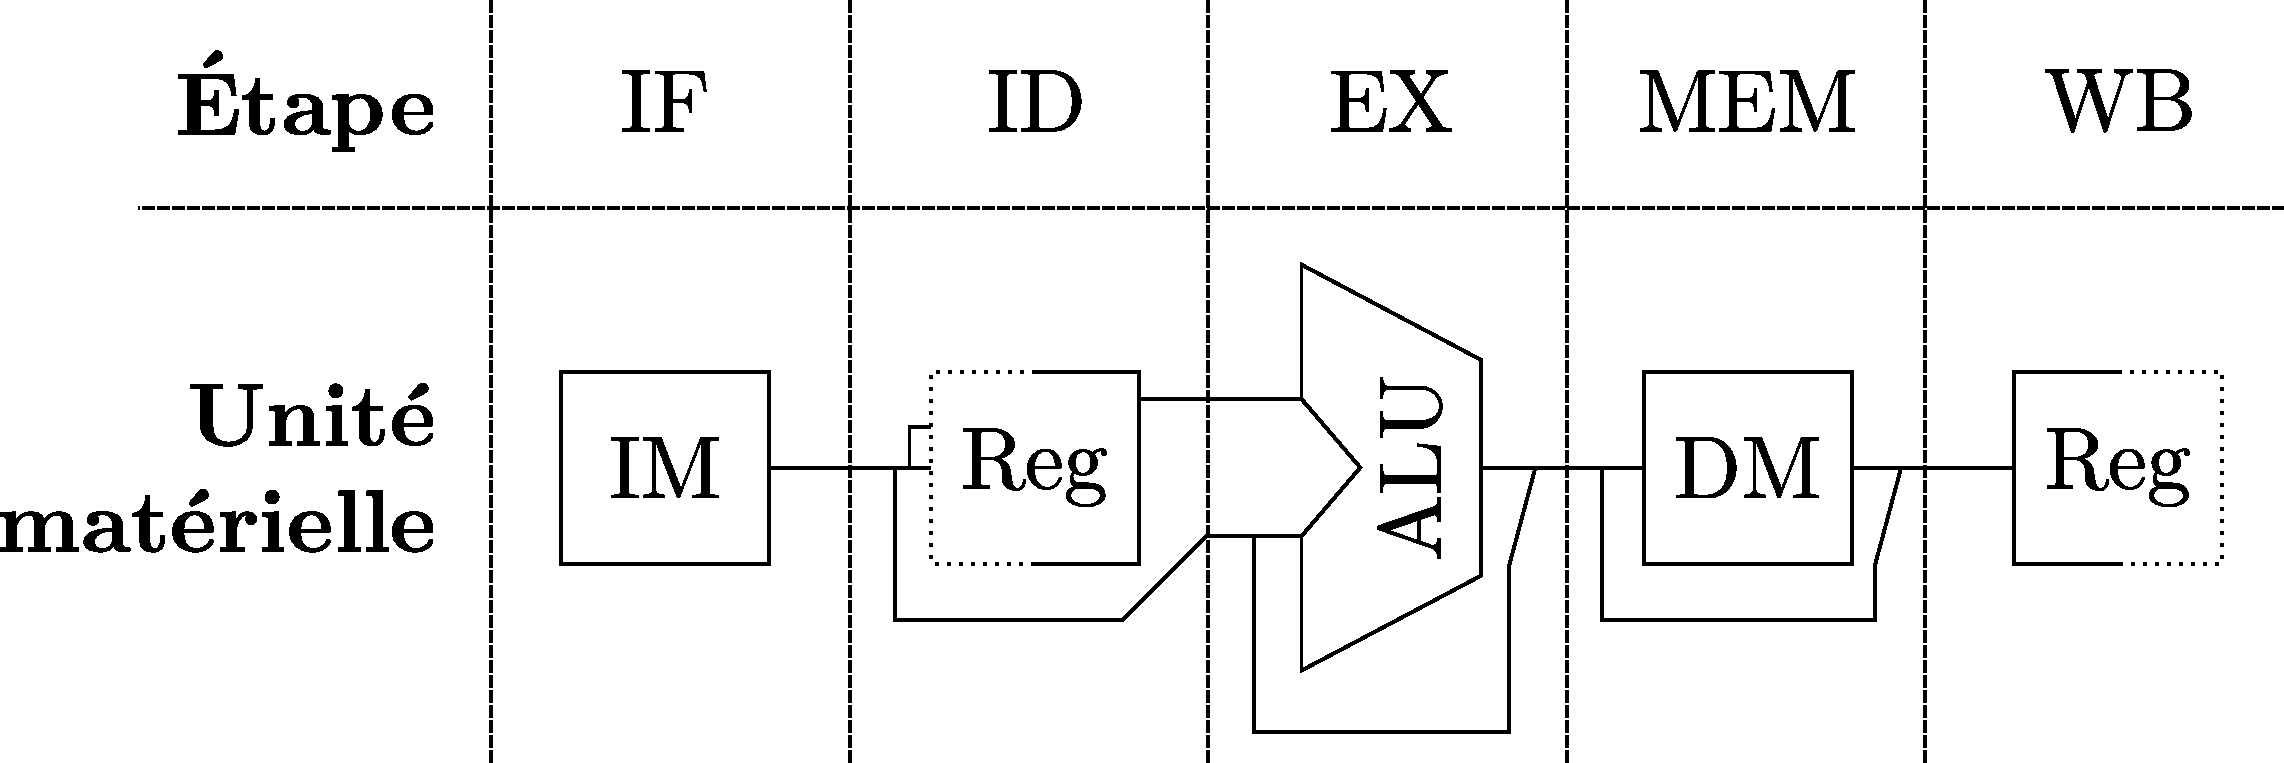
\includegraphics[width=\textwidth]{fig/stages}}
      \end{column}
    \end{columns}
  \end{minipage}
  \begin{figure}[htp]
    \centering
    \only<1-2>{
\includegraphics[width=\textwidth]{fig/frise1}}
    \only<3-4>{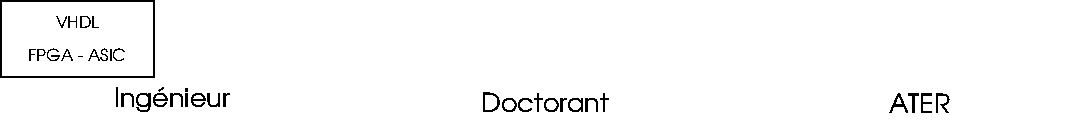
\includegraphics[width=\textwidth]{fig/frise2}}
    \only<5->{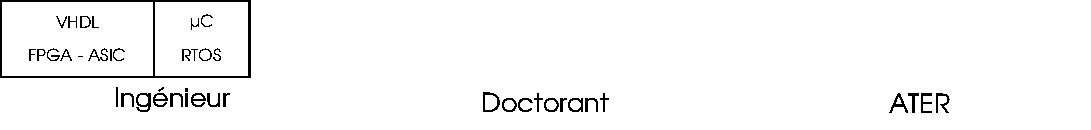
\includegraphics[width=\textwidth]{fig/frise3}}
  \end{figure}
\end{frame}
\begin{frame}[t]{Formation d'ingénieur - Apprentissage}
  \begin{minipage}[t][5.0cm][t]{\textwidth}
    \begin{columns}[T]
      \begin{column}{0.63\textwidth}
        \begin{itemize}
          \item<+-> Entreprise WorldCast Systems
          \item<+-> Broadcast
          \item<+-> \'Equipe R\&D émetteurs FM
          \begin{itemize}
            \item<+-> Conception de cartes électroniques
            \item<+-> Programmation de uC
            \item<+-> Interface graphique
          \end{itemize}
        \end{itemize}
      \end{column}
      \begin{column}{0.04\textwidth}

      \end{column}
      \begin{column}{0.33\textwidth}
        \only<1->{
\includegraphics[width=\textwidth]{fig/worldcast}\\}
        \only<3-5>{\vspace{0.8cm}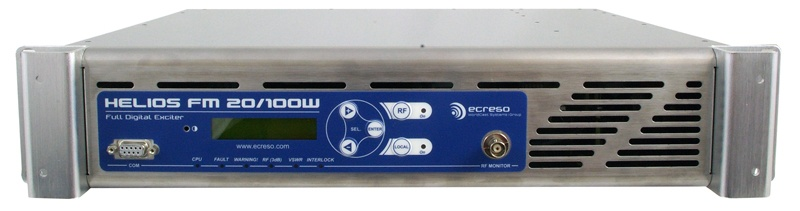
\includegraphics[width=\textwidth]{fig/helios}\\}
        \only<6->{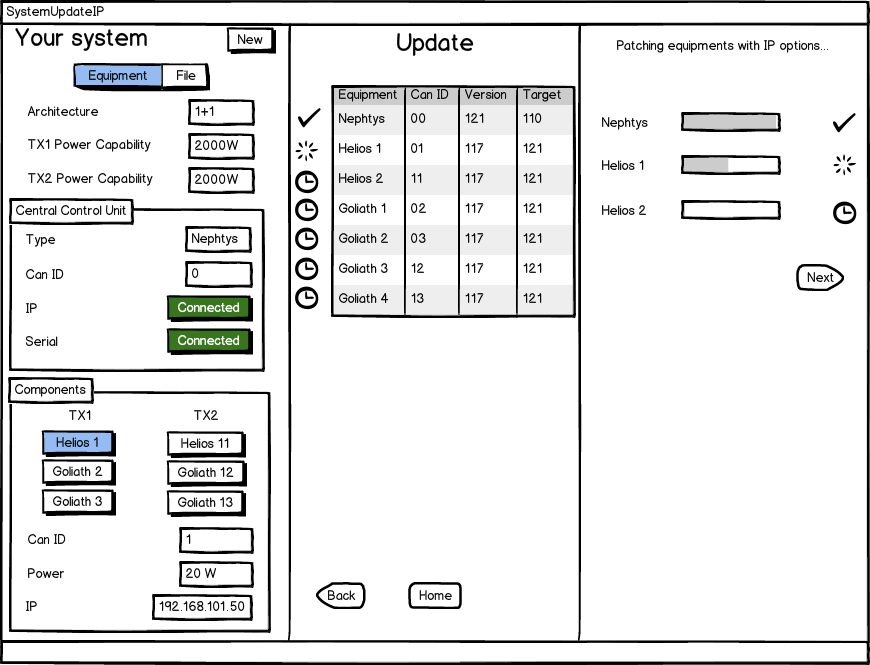
\includegraphics[width=\textwidth]{fig/engi}}
      \end{column}
    \end{columns}
  \end{minipage}
  \begin{figure}[htp]
    \centering
    \only<1-5>{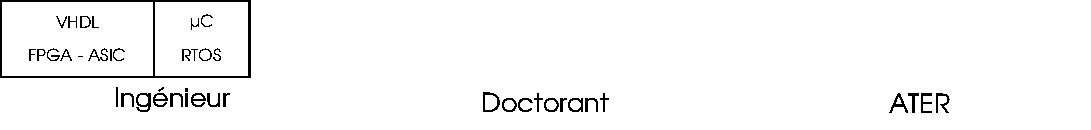
\includegraphics[width=\textwidth]{fig/frise3}}
    \only<6>{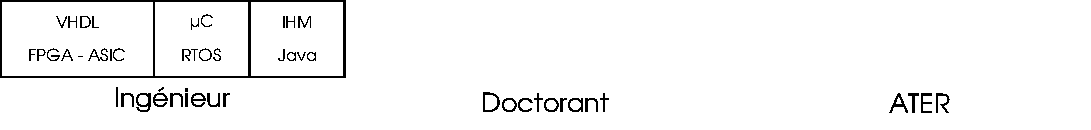
\includegraphics[width=\textwidth]{fig/frise4}}
  \end{figure}


\end{frame}

\subsection{Doctorat}
\begin{frame}[t]{Décodage de Codes Polaires}
  \begin{minipage}[t][5.0cm][t]{\textwidth}
  \vspace{1cm}
  \centering
  "Décodage de codes polaires sur des architectures programmables"
  \vspace{1cm}
    % \begin{columns}
      % \begin{column}{0.63\textwidth}
        % \vspace{-30pt}
          % \begin{itemize}
            % \item Décodage de codes polaires sur des architectures programmables
            % \item Cotutelle Canada - France
          % \end{itemize}
      % \end{column}
      % \begin{column}{0.04\textwidth}

    %   \end{column}
    %   \begin{column}{0.33\textwidth}
        
\includegraphics[width=0.25\textwidth]{logos/ims}\hspace{2cm}
        
\includegraphics[width=0.25\textwidth]{logos/poly2}
    %     \only<+->{\includegraphics[width=\textwidth]{fig/frise}}
    %   \end{column}
    % \end{columns}
  \end{minipage}
  \begin{figure}[htp]
    \centering
    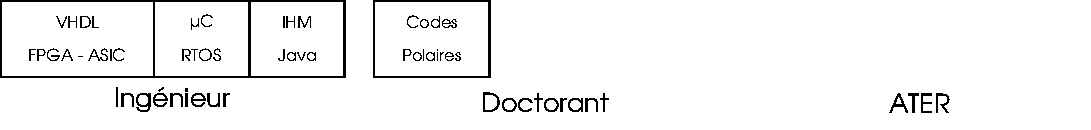
\includegraphics[width=\textwidth]{fig/frise5}
  \end{figure}
\end{frame}

\begin{frame}[t]{Implémentation logicielle SC Liste}
  \begin{minipage}[t][5.0cm][t]{\textwidth}
    \begin{columns}[T]
      \begin{column}{0.63\textwidth}
        \begin{itemize}
          \item<+-> Décodeurs logiciels - x86\_64 \& ARM
          \item<+-> Implémentation flexible et générique
          \item<+-> Parallélisation
          \begin{itemize}
            \item<3-> SIMD, multithreads, multinodes
          \end{itemize}
          \item<+-> Adaptatif le plus rapide à ce jour
          \item<+-> Intégré avec le projet AFF3CT
          \begin{itemize}
            \item<5-> \url{https://aff3ct.github.io}
          \end{itemize}
        \end{itemize}
      \end{column}
      \begin{column}{0.04\textwidth}

      \end{column}
      \begin{column}{0.33\textwidth}
        \only<1->{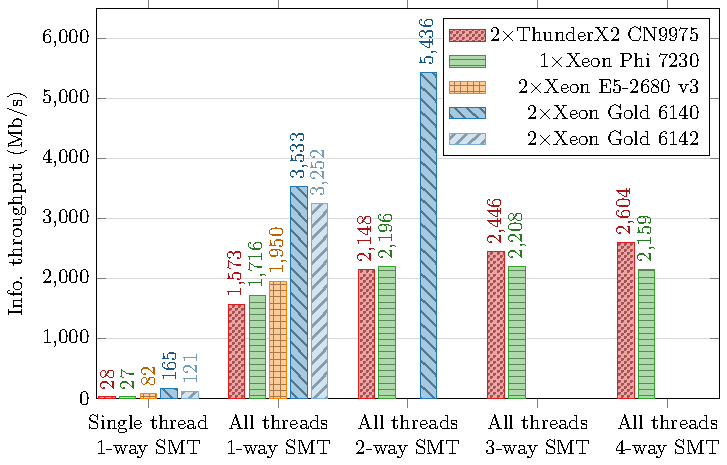
\includegraphics[width=\textwidth]{fig/throughput}\\ \vspace{0.5cm}}
        \only<5->{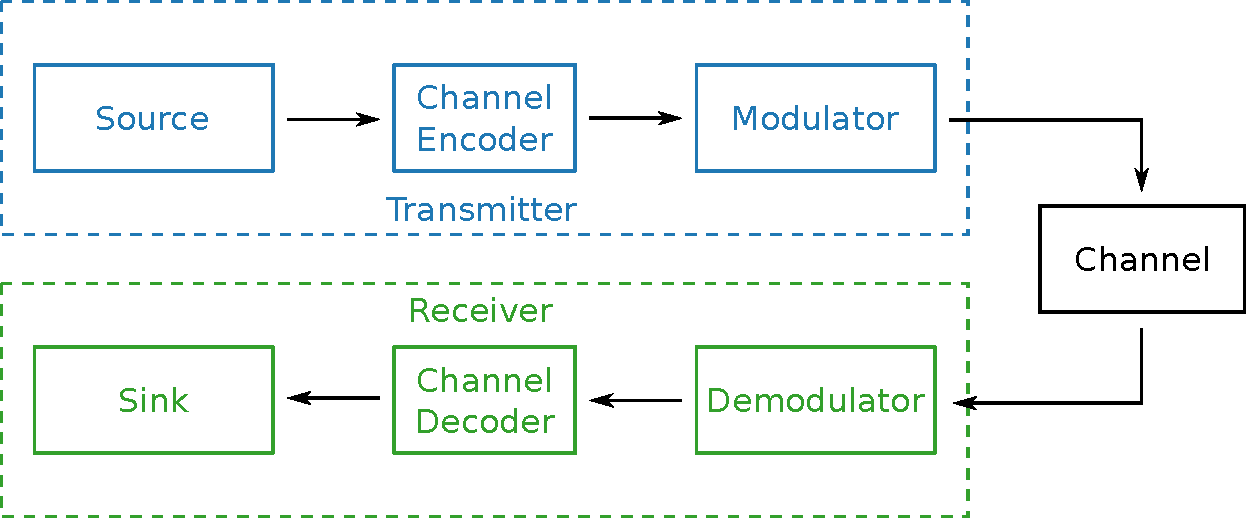
\includegraphics[width=\textwidth]{fig/chain_ink}}
      \end{column}
    \end{columns}
  \end{minipage}
    \begin{figure}[htp]
    \centering
    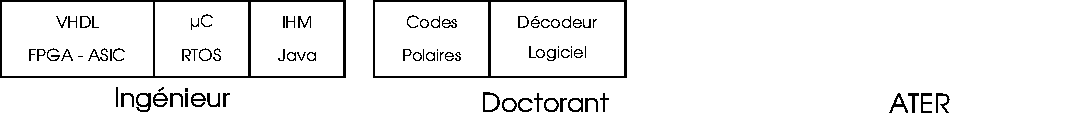
\includegraphics[width=\textwidth]{fig/frise6}
  \end{figure}
\end{frame}

\begin{frame}[t]{Architectures ASIP pour le décodage de codes polaires}
  \begin{minipage}[t][5.0cm][t]{\textwidth}
    \begin{columns}[T]
      \begin{column}{0.56\textwidth}
        \begin{itemize}
          \item<+-> Architecture 1 - Tensilica
          \begin{itemize}
            \item<1-> Collaboration Pierre Langlois (Polytechnique Montréal)
          \end{itemize}
          \vspace{1.5cm}
          \item<+-> Architecture 2 - TTA
          \begin{itemize}
            \item<2-> Collaboration Pekka Jääskeläinen (TUT)
          \end{itemize}
        \end{itemize}
      \end{column}
      \begin{column}{0.04\textwidth}

      \end{column}
      \begin{column}{0.40\textwidth}
        \only<1-2>{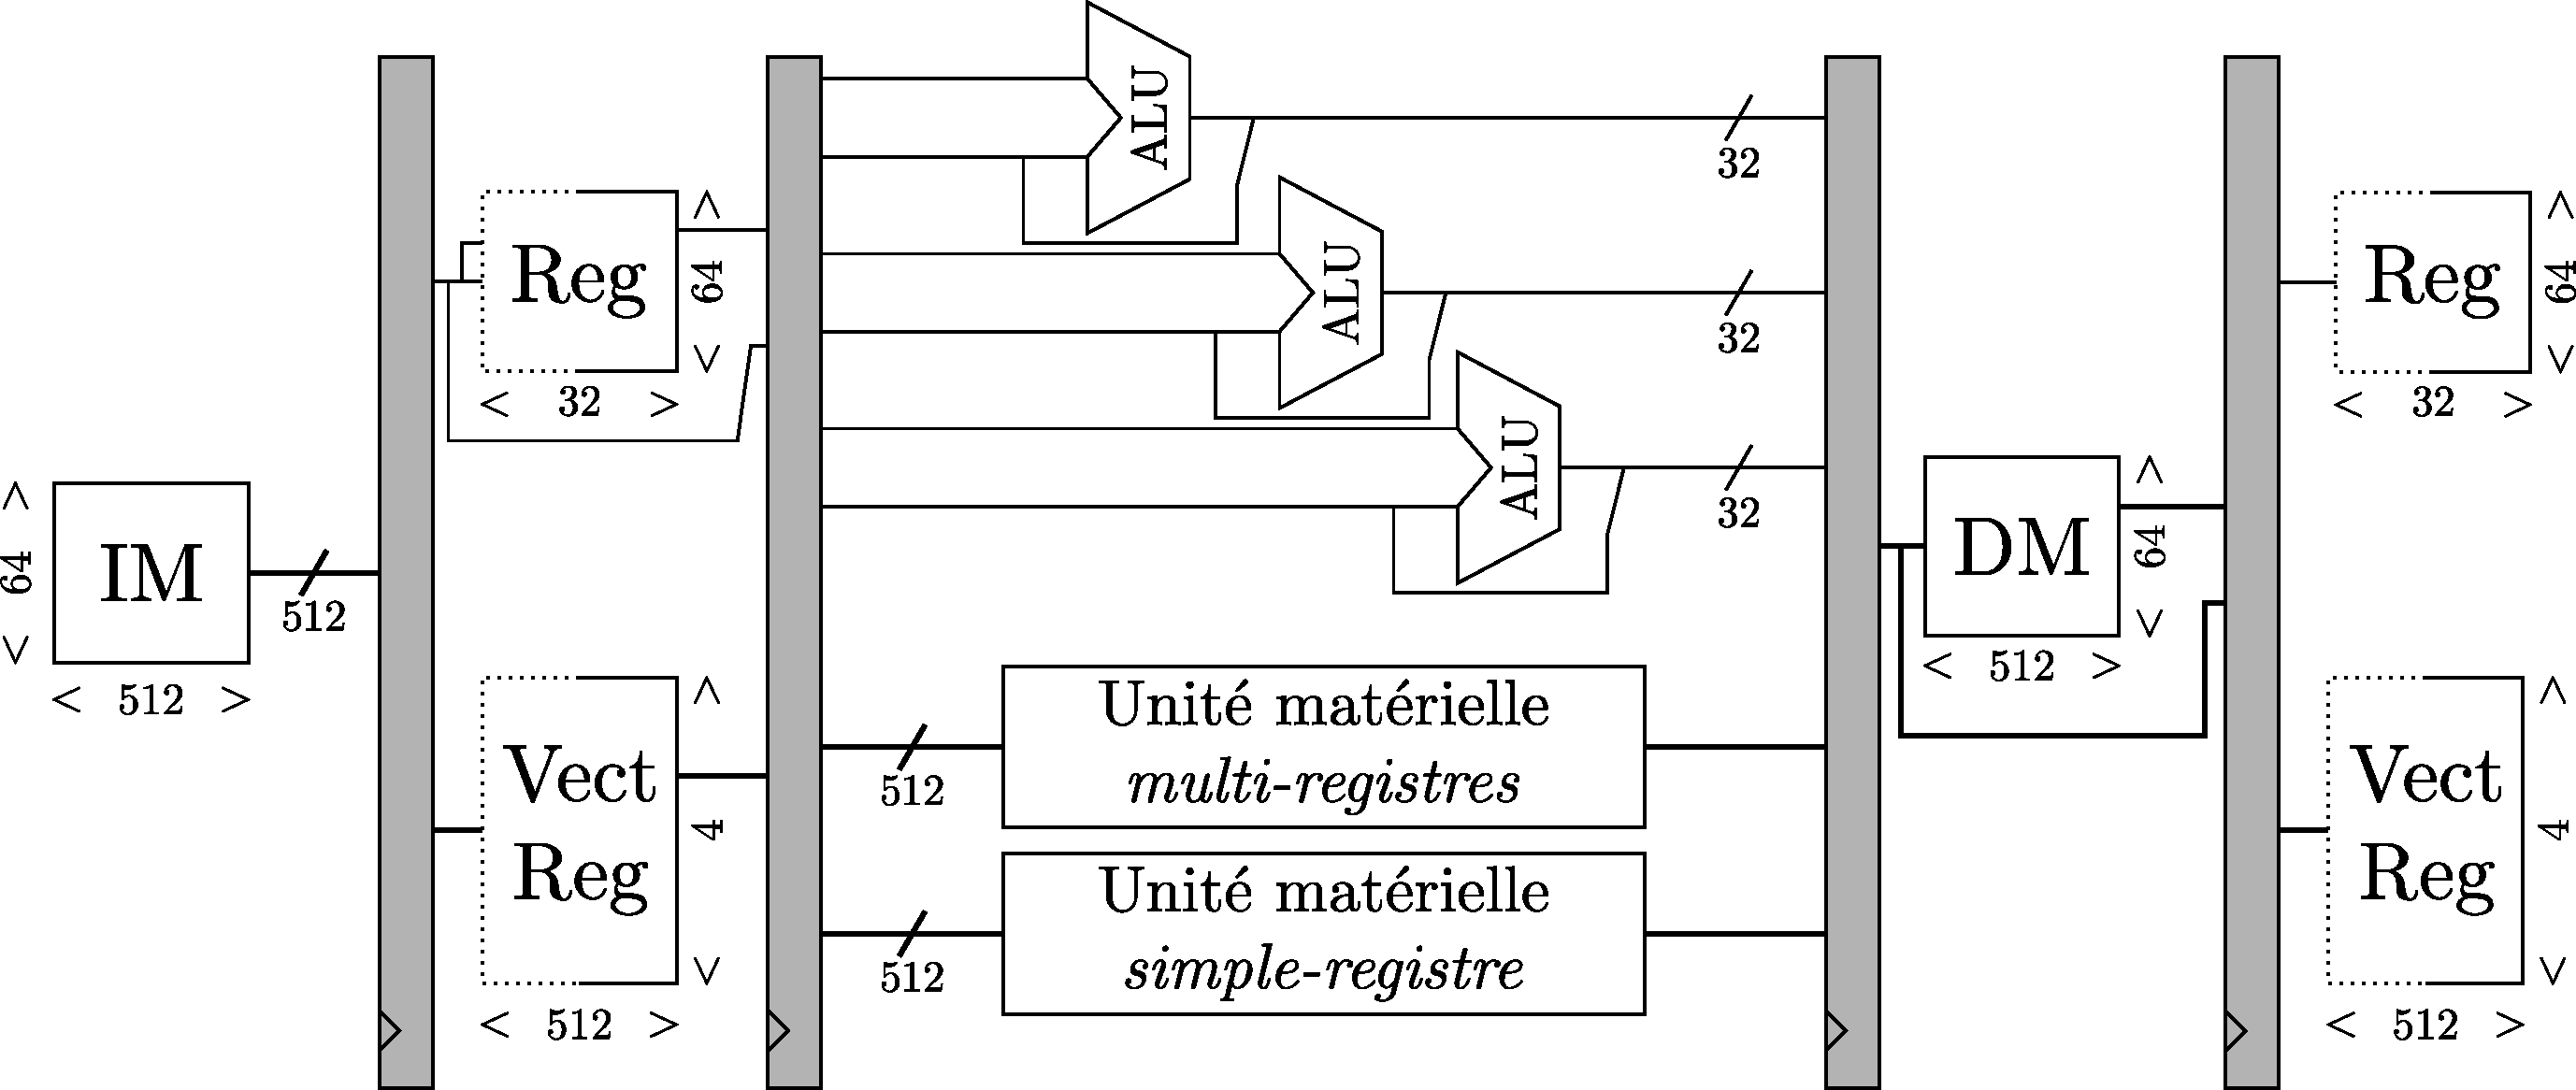
\includegraphics[width=\textwidth]{fig/full_tensilica}\\ \vspace{0.5cm}}
        \only<2>{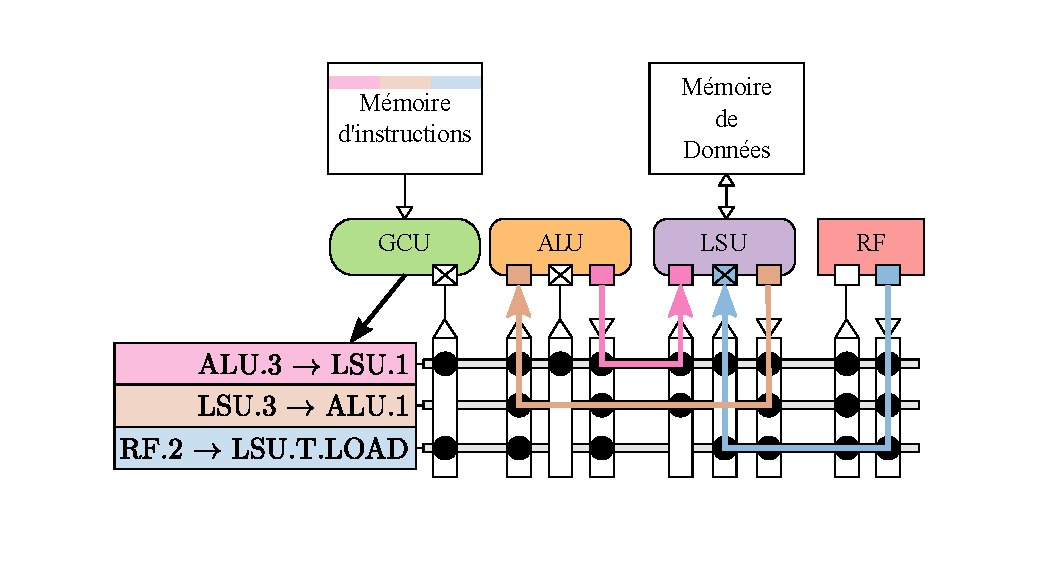
\includegraphics[width=\textwidth]{fig/tta_base}}
            \only<3>{
            \vspace{-0.5cm}
    \begin{table}
      \centering
      {
      \small\resizebox{\linewidth}{!}{
      \begin{tabular}{c|c|c|c|c}
        \toprule

        Architecture & $N$ & \begin{tabular}{c}Latence\\{[$\mu$s]}\end{tabular} & \begin{tabular}{c}Débit\\{[Mb/s]}\end{tabular} & \begin{tabular}{c}$E_b$\\{[nJ/bit]}\end{tabular} \\

        \cmidrule(lr){1-1}
        \cmidrule(lr){2-2}
        \cmidrule(lr){3-5}


        \multirow{2}{*}{\bf i7-3.3GHz}              & $1024$   & $2.0$  & \GREEN{$\mathbf{257}$} & \RED{$\mathbf{41}$}   \\
                                                    & $512$    & $1.2$  & \GREEN{$\mathbf{210}$} & \RED{$\mathbf{49}$}   \\
        \multirow{2}{*}{\bf (GPP)}                  & $256$    & $0.7$  & \GREEN{$\mathbf{179}$} & \RED{$\mathbf{59}$}   \\
                                                    & $128$    & $0.4$  & \GREEN{$\mathbf{143}$} & \RED{$\mathbf{73}$}   \\
        \midrule
        \multirow{2}{*}{\bf A57-1.1GHz}             & $1024$   & $10.7$ & \ORANGE{$\mathbf{48}$} & \RED{$\mathbf{17}$}   \\
                                                    & $512$    & $5.3$  & \ORANGE{$\mathbf{48}$} & \RED{$\mathbf{17}$}   \\
        \multirow{2}{*}{\bf (GPP)}                  & $256$    & $2.8$  & \ORANGE{$\mathbf{46}$} & \RED{$\mathbf{17}$}   \\
                                                    & $128$    & $1.6$  & \ORANGE{$\mathbf{41}$} & \RED{$\mathbf{20}$}   \\
        \midrule
        \multirow{2}{*}{\bf LX7-835MHz}             & $1024$   & $7.2$  & \ORANGE{$\mathbf{71}$} & \ORANGE{$\mathbf{1.6}$}  \\
                                                    & $512$    & $3.9$  & \ORANGE{$\mathbf{66}$} & \ORANGE{$\mathbf{1.7}$}  \\
        \multirow{2}{*}{\bf (ASIP)}                 & $256$    & $1.9$  & \ORANGE{$\mathbf{65}$} & \ORANGE{$\mathbf{1.7}$}  \\
                                                    & $128$    & $1.0$  & \ORANGE{$\mathbf{62}$} & \ORANGE{$\mathbf{1.8}$}  \\
        \midrule
        \multirow{2}{*}{\bf TTPD-800MHz}            & $1024$   & $1.4$  & \GREEN{$\mathbf{352}$} & \GREEN{$\mathbf{0.14}$} \\ % 1512 cycles
                                                    & $512$    & $0.8$  & \GREEN{$\mathbf{313}$} & \GREEN{$\mathbf{0.15}$} \\ % 803 cycles
        \multirow{2}{*}{\bf (ASIP)}                 & $256$    & $0.4$  & \GREEN{$\mathbf{304}$} & \GREEN{$\mathbf{0.16}$} \\ % 413 cycles
                                                    & $128$    & $0.2$  & \GREEN{$\mathbf{284}$} & \GREEN{$\mathbf{0.17}$} \\ % 224 cycles

        \bottomrule
      \end{tabular}
      }}
    \end{table}
    }


      \end{column}
    \end{columns}
  \end{minipage}
  \begin{figure}[htp]
    \centering
    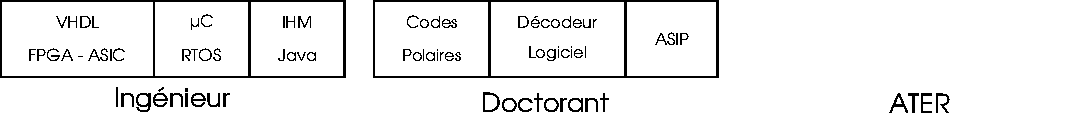
\includegraphics[width=\textwidth]{fig/frise7}
  \end{figure}
\end{frame}

\subsection{Poste ATER}
\begin{frame}[t]{Enseignement}
  \begin{minipage}[t][5.0cm][t]{\textwidth}
    \vspace{-0.5cm}
    \begin{itemize}
      \item<+-> \'Electronique numérique \\
    \end{itemize}
    \small{
      \begin{tabular}{ l l l l }
      Logique combinatoire s\'equentielle & 32 HETD & 1A & Bases       \\
      Projet de conception en \'electronique         & 50 HETD & 1A & VHDL - FPGA \\
      Architecture reconfigurable                    & 20 HETD & 2A & VHDL - FPGA \\
      \'Electronique Num\'erique                     & 25 HETD & 1A & VHDL - FPGA
    \end{tabular}
    }
    \vspace{0cm}
    \begin{itemize}
      \item<+-> Informatique
    \end{itemize}
    \only<2>
    {
      \small{
      \begin{tabular}{ l l l l }
        Architecture des ordinateurs     & 16 HETD & 1A & Archi  \\
        Projet micro-processeur          & 36 HETD & 2A & C      \\
        Projet micro-informatique        & 42 HETD & 2A & C - OS \\
        Programmation objet. Langage C++ & 15 HETD & 2A & C++
      \end{tabular}
      }
    }
  \end{minipage}
  \begin{figure}[htp]
    \centering
    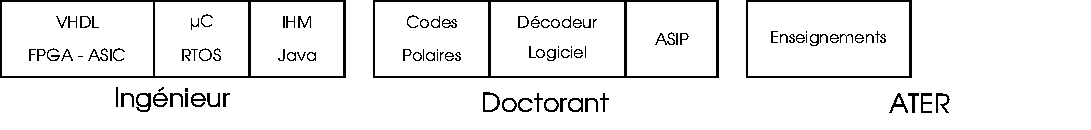
\includegraphics[width=\textwidth]{fig/frise8}
  \end{figure}
\end{frame}

\begin{frame}[t]{Travaux}
 \begin{minipage}[t][5.0cm][t]{\textwidth}
    \begin{columns}[T]
      \begin{column}{0.63\textwidth}
          \begin{itemize}
            \item Projet industriel (Airbus Defense \& Space)
            \begin{itemize}
              \item Radio logicielle
              \item Communications satellitaires
            \end{itemize}
          \end{itemize}
      \end{column}
      \begin{column}{0.04\textwidth}

      \end{column}
      \begin{column}{0.33\textwidth}
        \only<+->{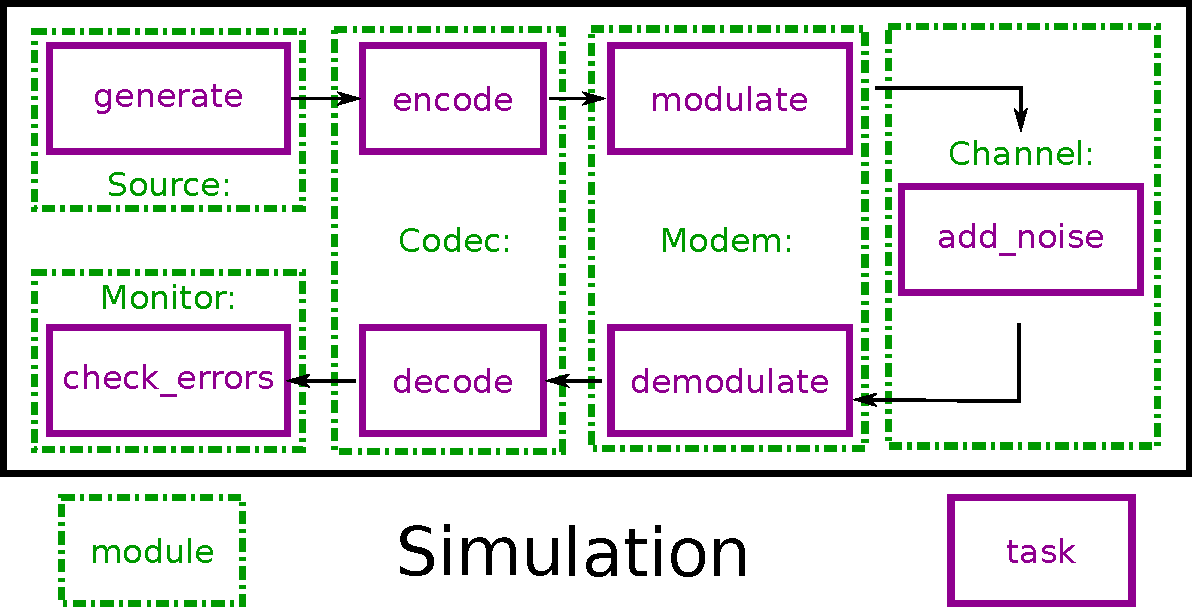
\includegraphics[width=\textwidth]{fig/chaine_airbus}}
      \end{column}
    \end{columns}
  \end{minipage}
  \begin{figure}[htp]
    \centering
    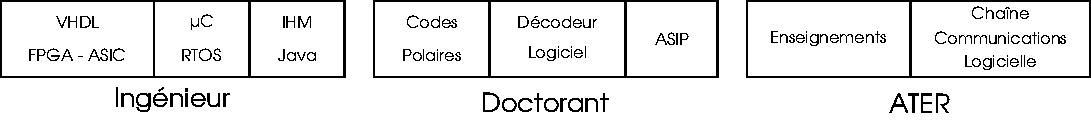
\includegraphics[width=\textwidth]{fig/frise9}
  \end{figure}
\end{frame}


\begin{frame}[c]{Publications}

  \begin{enumerate}
\renewcommand{\section}[2]{} % Trick to avoid references section

    \renewcommand*{\bibfont}{\scriptsize}
    \nocite{leonardon_fast_2017,leonardon_custom_2018,ghaffari_improving_2017,leonardon_tta_2018,Ghaffari2018,cassagne_fast_2017,cassagne_gdr_2017,leonardon_custom_2018}
    \vfill
    \item<+-> Implémentation logicielle de l'algorithme  SCL
    \scriptsize{\printbibliography[keyword={fast-scl}]}
    \vfill
    \item<+-> Spécialisation d'un processeur Tensilica
    \scriptsize{\printbibliography[keyword={tensilica}]}
    \vfill
    \item<+-> Conception d'un processeur de type TTA
    \scriptsize{\printbibliography[keyword={tta}]}
    \vfill
  \end{enumerate}

\end{frame}

\begin{frame}[c]{Publications}

  \begin{enumerate}
\renewcommand{\section}[2]{} % Trick to avoid references section

    \renewcommand*{\bibfont}{\scriptsize}
    \nocite{leonardon_fast_2017,leonardon_custom_2018,ghaffari_improving_2017,leonardon_tta_2018,leonardon_tta_2019,Ghaffari2018,cassagne_fast_2017,cassagne_gdr_2017,cassagne2019aff3ct}
    \vfill
    \item<+-> Implémentation du décodeur SCMA
    \printbibliography[keyword={ghaffari}]
    \vfill
    \item<+-> Contribution au projet AFF3CT
    \printbibliography[keyword={aff3ct}]
    \vfill
  \end{enumerate}

\end{frame}





\section{Intégration}
\subsection{Enseignement}
\begin{frame}[t]{Enseignements de première année}
  \begin{minipage}[t][5.0cm][t]{\textwidth}
    \begin{columns}[T]
      \begin{column}{0.63\textwidth}
          \begin{itemize}
            \item<+-> Opérationnel sur l'enseignement d'électronique numérique,
            \item<+-> Apte à encadrer les différents projets (FAIRE, SAR, CODEV).
          \end{itemize}
      \end{column}
      \begin{column}{0.04\textwidth}

      \end{column}
      \begin{column}{0.33\textwidth}
        \only{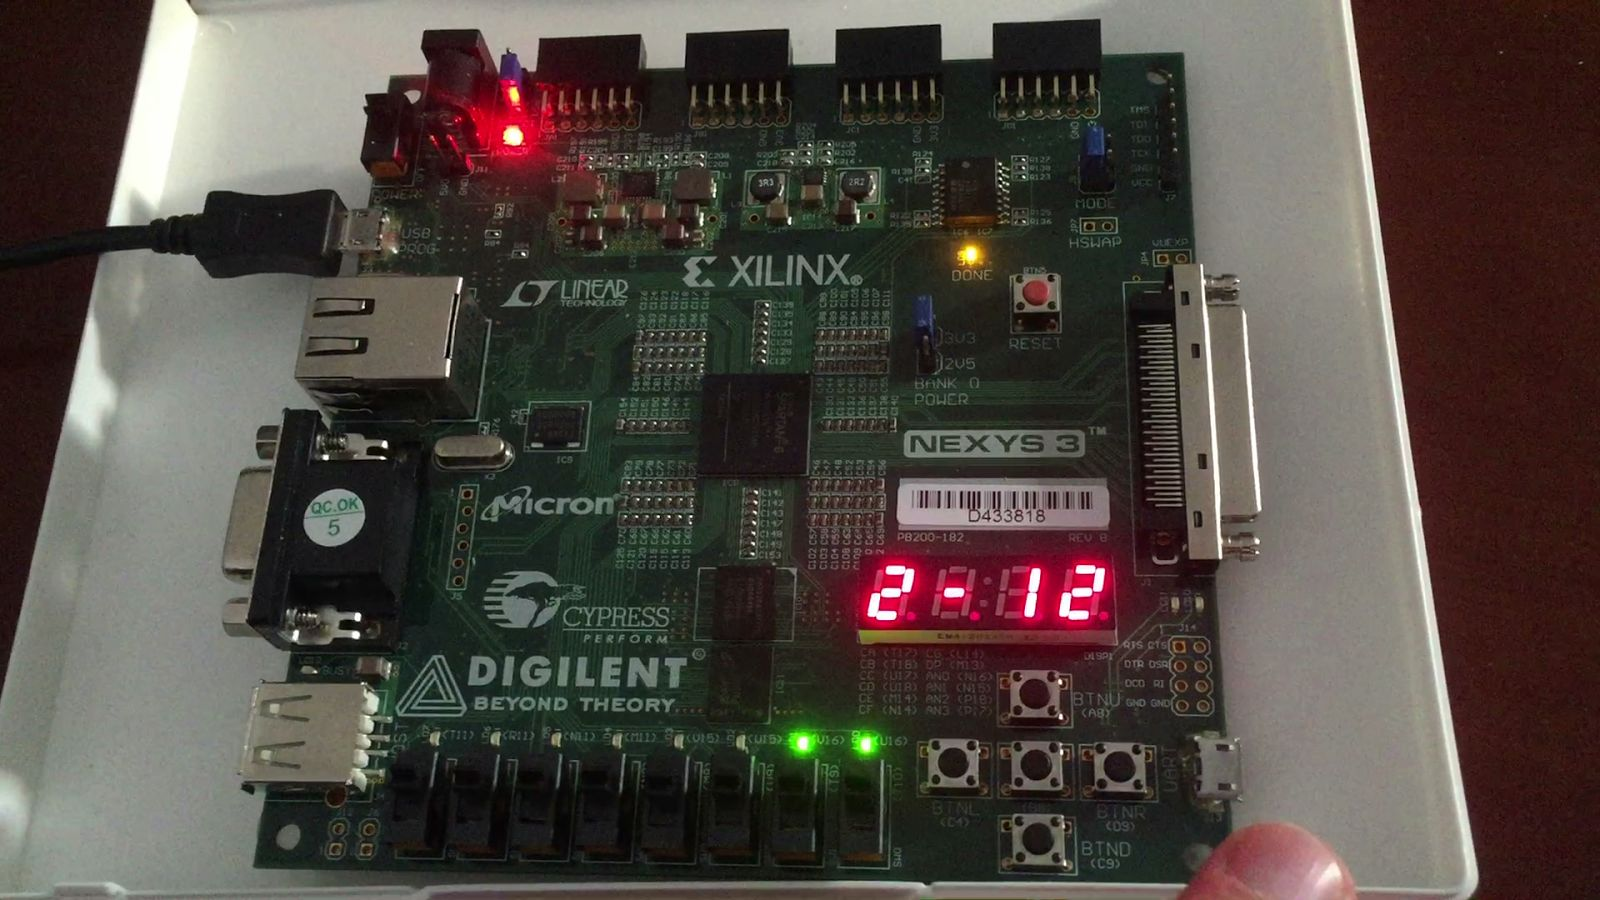
\includegraphics[width=\textwidth]{fig/loto}}
      \end{column}
    \end{columns}
  \end{minipage}
  \begin{figure}[htp]
    \centering
    \only<1>{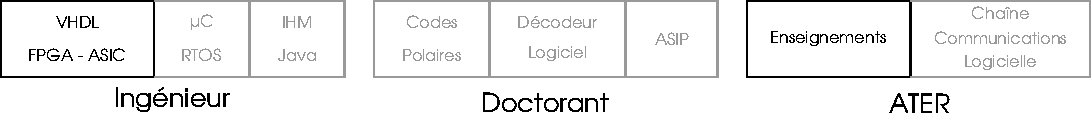
\includegraphics[width=\textwidth]{fig/frise10}}
    \only<2>{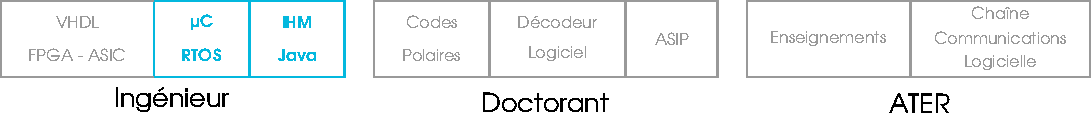
\includegraphics[width=\textwidth]{fig/frise11}}
  \end{figure}


\end{frame}

\begin{frame}[t]{TAF Systèmes Embarqués Hétérogènes}
  \begin{minipage}[t][5.0cm][t]{\textwidth}
  \centering
  \vspace{0.8cm}
    « La double compétence \BLUE{logicielle} et \RED{matérielle}, indissociable des systèmes embarqués, est très recherchée. »
  \end{minipage}
  \begin{figure}[htp]
    \centering
    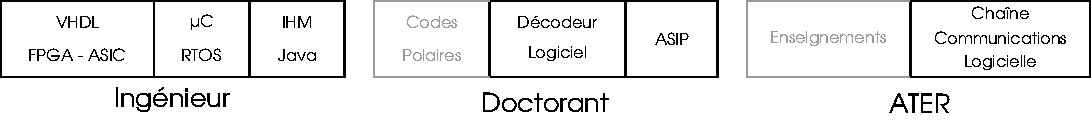
\includegraphics[width=\textwidth]{fig/frise12}
  \end{figure}
\end{frame}

\begin{frame}[t]{UE Coeurs}
  \begin{minipage}[t][5.0cm][t]{\textwidth}
    \begin{columns}[T]
      \begin{column}{0.63\textwidth}
        \begin{itemize}
            \item<+-> UEC1 : Circuits intégrés numériques et analogiques
            \item<+-> UEC2 : Méthodologies - de l’algorithme à la puce
            \item<+-> UEC3 : Systèmes embarqués
        \end{itemize}
      \end{column}
      \begin{column}{0.04\textwidth}

      \end{column}
      \begin{column}{0.33\textwidth}
        \only<1>{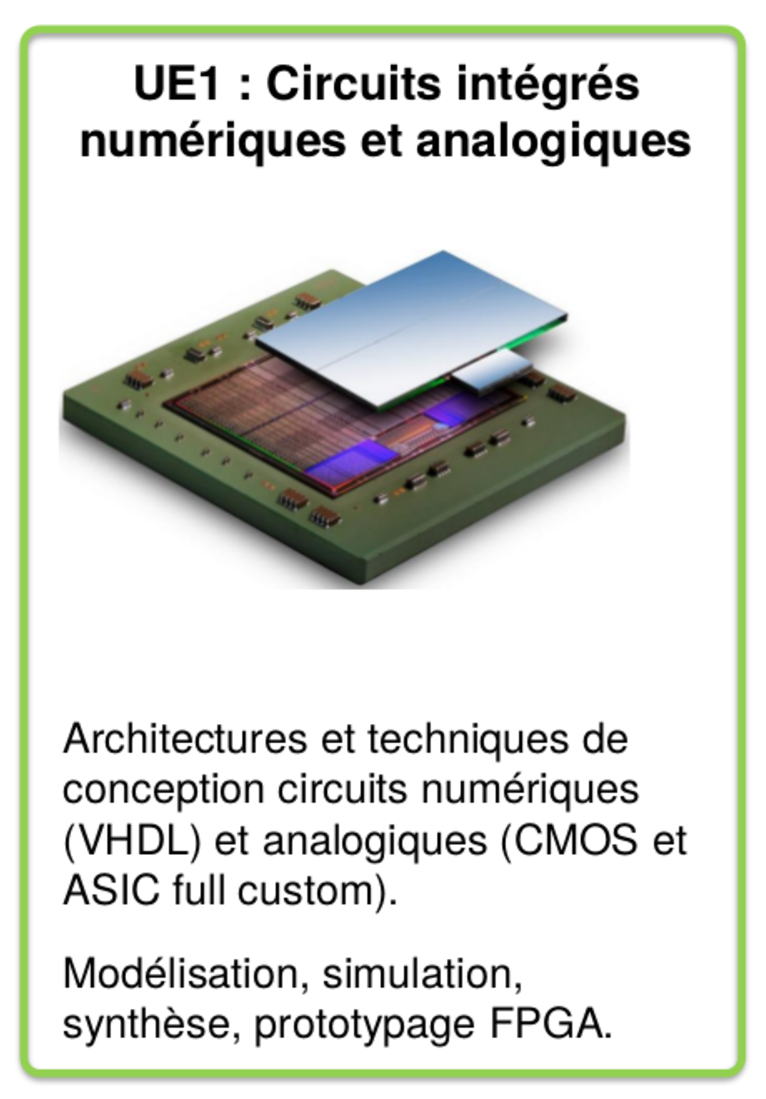
\includegraphics[width=.9\textwidth]{fig/UEC1}}
        \only<2>{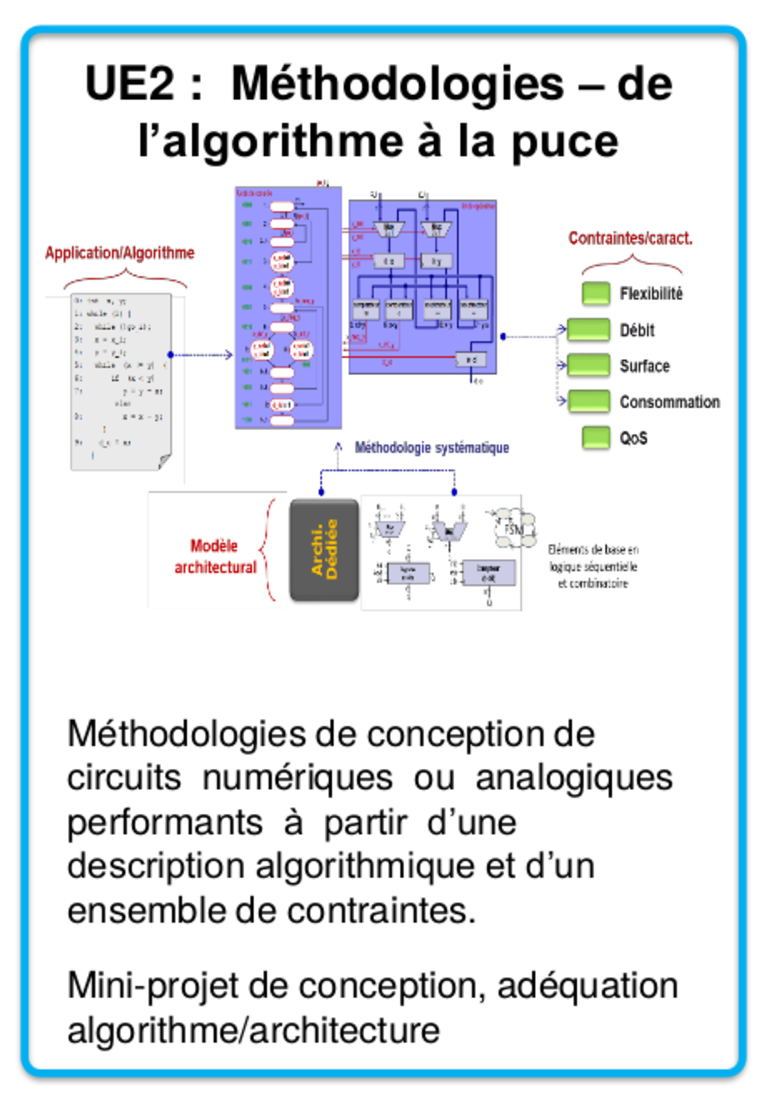
\includegraphics[width=.9\textwidth]{fig/UEC2}}
        \only<3>{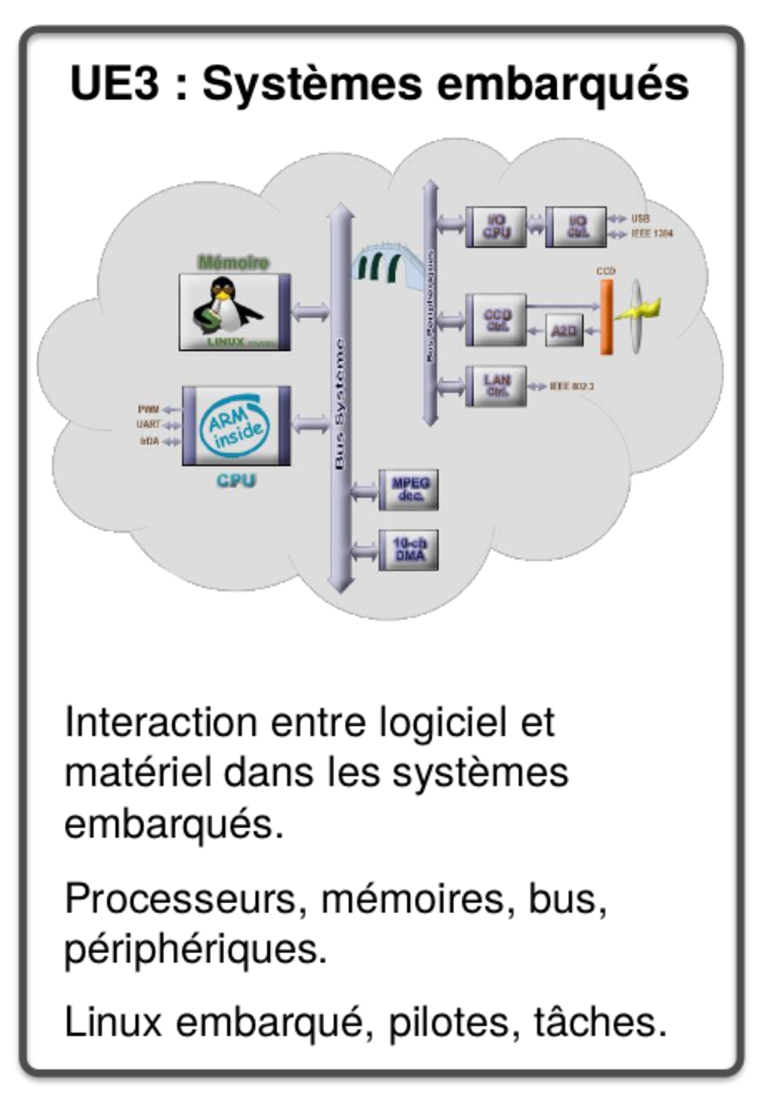
\includegraphics[width=.9\textwidth]{fig/UEC3}}
      \end{column}
    \end{columns}
  \end{minipage}
  \begin{figure}[htp]
    \centering
    \only<1>{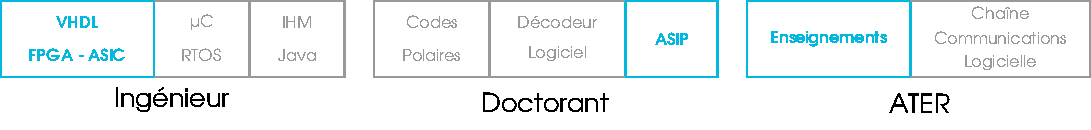
\includegraphics[width=\textwidth]{fig/frise13}}
    \only<2>{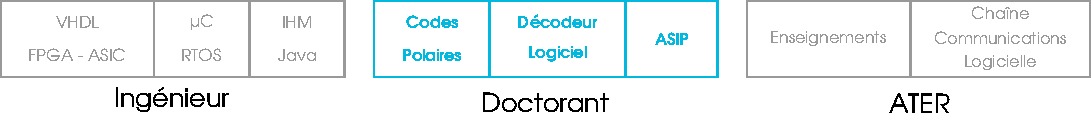
\includegraphics[width=\textwidth]{fig/frise14}}
    \only<3>{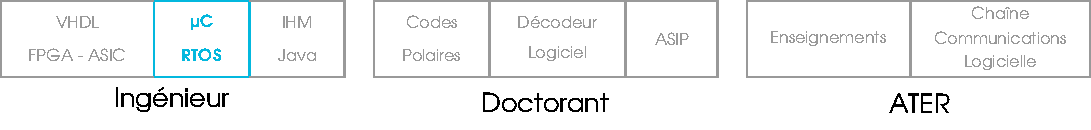
\includegraphics[width=\textwidth]{fig/frise15}}
  \end{figure}


\end{frame}

\begin{frame}[t]{UE \'Electives}
  \begin{minipage}[t][5.0cm][t]{\textwidth}
    \begin{columns}[T]
      \begin{column}{0.63\textwidth}
        \begin{itemize}
            \item<+-> UEE : Conception haut niveau de circuits
            \item<+-> UEE : IA Intro \& IA Optimisation
            \item<+-> UEE : Calcul parallèle
        \end{itemize}
      \end{column}
      \begin{column}{0.04\textwidth}

      \end{column}
      \begin{column}{0.33\textwidth}
        \only<1>{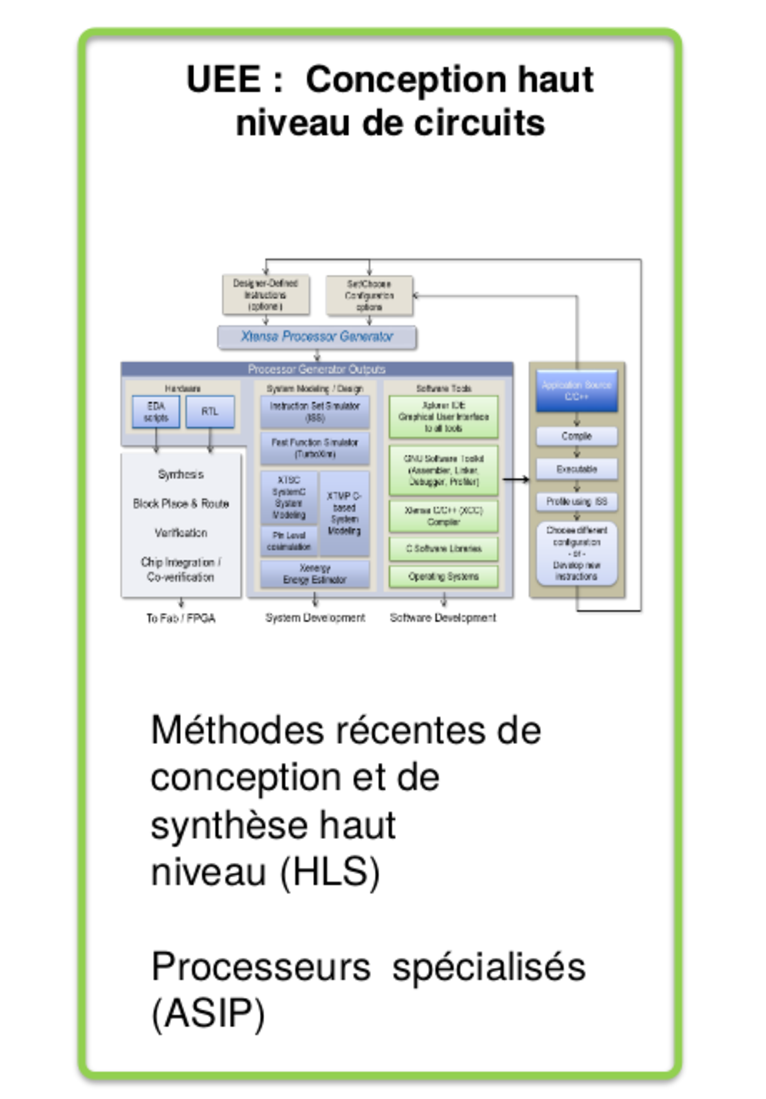
\includegraphics[width=.9\textwidth]{fig/UEE1}}
        \only<2>{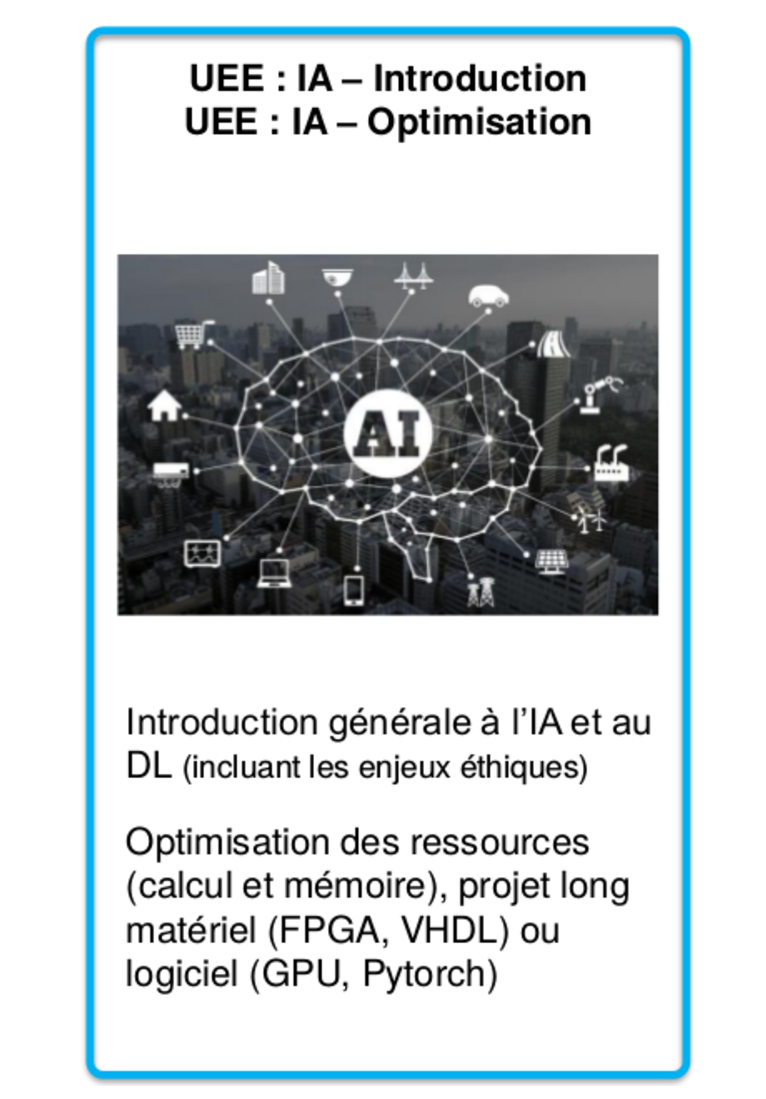
\includegraphics[width=.9\textwidth]{fig/UEE3}}
        % \only<3>{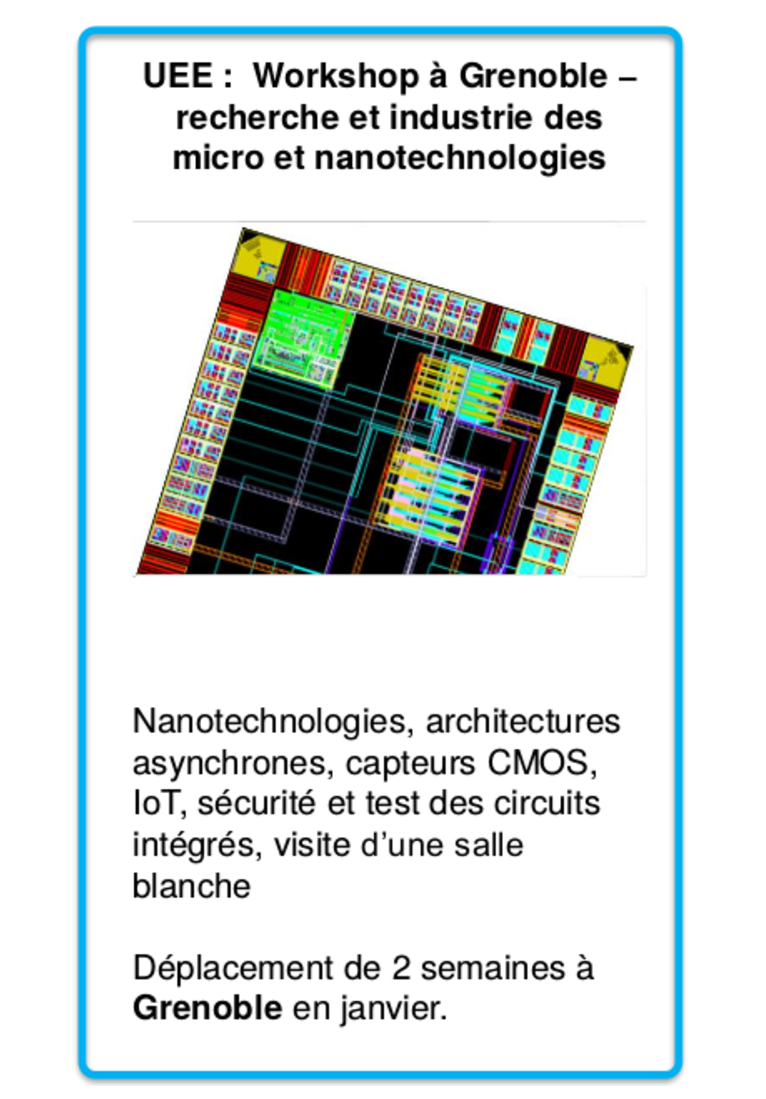
\includegraphics[width=.9\textwidth]{fig/UEE4}}
        \only<3>{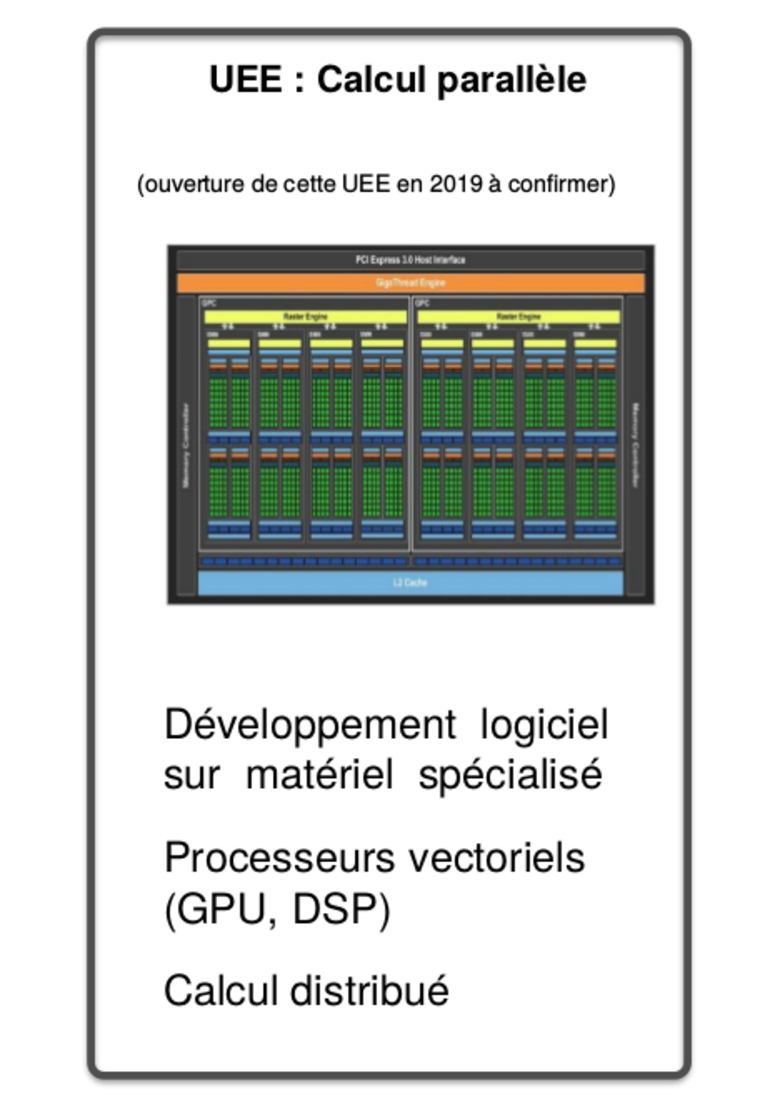
\includegraphics[width=.9\textwidth]{fig/UEE2}}
      \end{column}
    \end{columns}
  \end{minipage}
  \begin{figure}[htp]
    \centering
    \only<1>{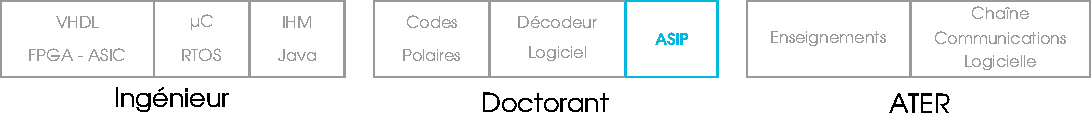
\includegraphics[width=\textwidth]{fig/frise16}}
    \only<2>{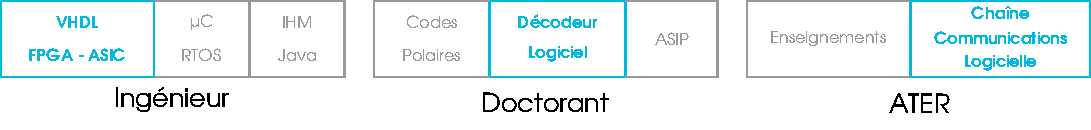
\includegraphics[width=\textwidth]{fig/frise17}}
    % \only<3>{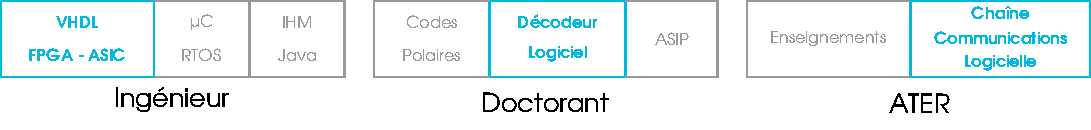
\includegraphics[width=\textwidth]{fig/frise17}}
    \only<3>{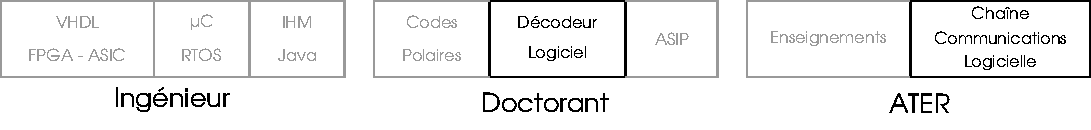
\includegraphics[width=\textwidth]{fig/frise18}}
  \end{figure}



\end{frame}


\begin{frame}[t]{TAF CoOC}
  \begin{minipage}[t][5.0cm][t]{\textwidth}
        \begin{itemize}
          \item Conception d'Objets Communicants
          \item Conception centrée sur l'utilisateur
          \item Prototypage rapide et développement agile
          \item L'objet dans son environnement
          \item Projet fil rouge
          \begin{itemize}
            \item Maquettage
            \item \'Etude des utilisateurs
            \item Rédaction cahier des charges
          \end{itemize}
        \end{itemize}
  \end{minipage}
  \begin{figure}[htp]
    \centering
    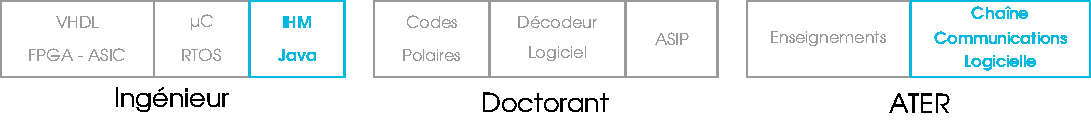
\includegraphics[width=\textwidth]{fig/frise25}
  \end{figure}
\end{frame}

\subsection{Recherche}
\begin{frame}[t]{Plan}
  \centering
  \tableofcontents[
    currentsection,
    currentsubsection,
    sectionstyle=show/show,
    subsectionstyle=show/shaded/shaded,
  ]
\end{frame}

\begin{frame}[t]{Axe de recherche 1 : Maintenance prédictive}

  \begin{minipage}[t][5.0cm][t]{\textwidth}
    \vspace*{-0.5cm}
    \begin{figure}[htp]
      \centering
      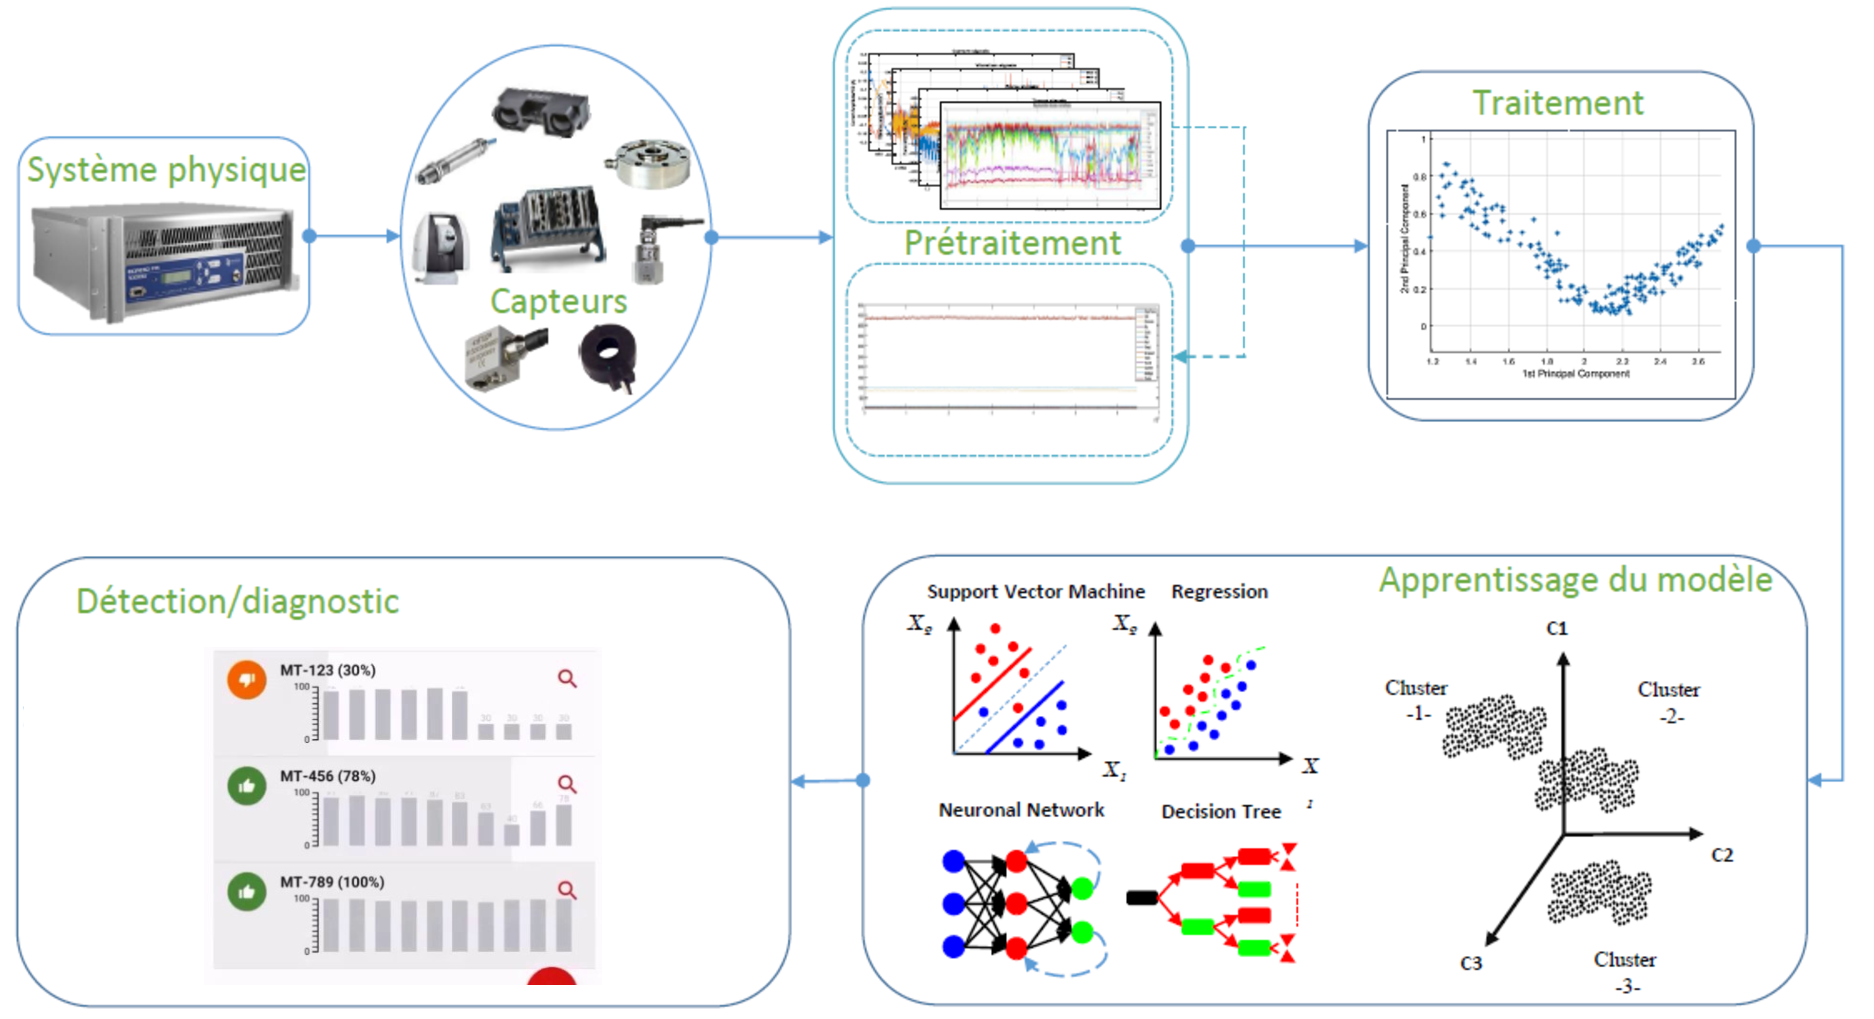
\includegraphics[width=0.8\textwidth]{fig/research/worldcast/phm.pdf}
    \end{figure}
  \end{minipage}
  \begin{figure}[htp]
    \centering
    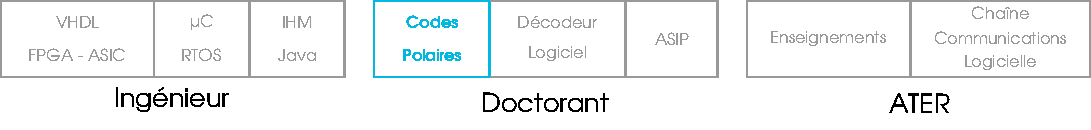
\includegraphics[width=\textwidth]{fig/frise20}
  \end{figure}
\end{frame}

\begin{frame}[t]{Axe de recherche 1 : Maintenance prédictive}
  \begin{minipage}[t][5.0cm][t]{\textwidth}
    \only<+>{
      \begin{columns}[T]
        \begin{column}{0.63\textwidth}
            \vspace*{1cm}
            \begin{itemize}
              \item Entreprise Worldcast Systems
              \item Premiers résultats
              \item Proposition CIFRE
              \item Prochaine étape : Kybio
          \end{itemize}
          \end{column}
        \begin{column}{0.04\textwidth}
        \end{column}
        \begin{column}{0.33\textwidth}
          
\includegraphics[width=\textwidth]{fig/research/worldcast/worldcast.png}
        \end{column}
      \end{columns}
    }

    \only<4>{
      \begin{figure}[t]
        
\includegraphics[width=0.3\textwidth]{fig/research/worldcast/worldcast_cut}
      \end{figure}
      \begin{itemize}
          \item Extraire automatiquement des données de surveillance SNMP,
          \item réaliser l'interface avec logiciel Kybio,
          \item proposer des algorithmes de prédiction,
          \item les appliquer et les évaluer sur les données recueillies.
      \end{itemize}
    }

    \begin{figure}[htp]
      \centering
      \only<+>{\vspace*{-0.5cm}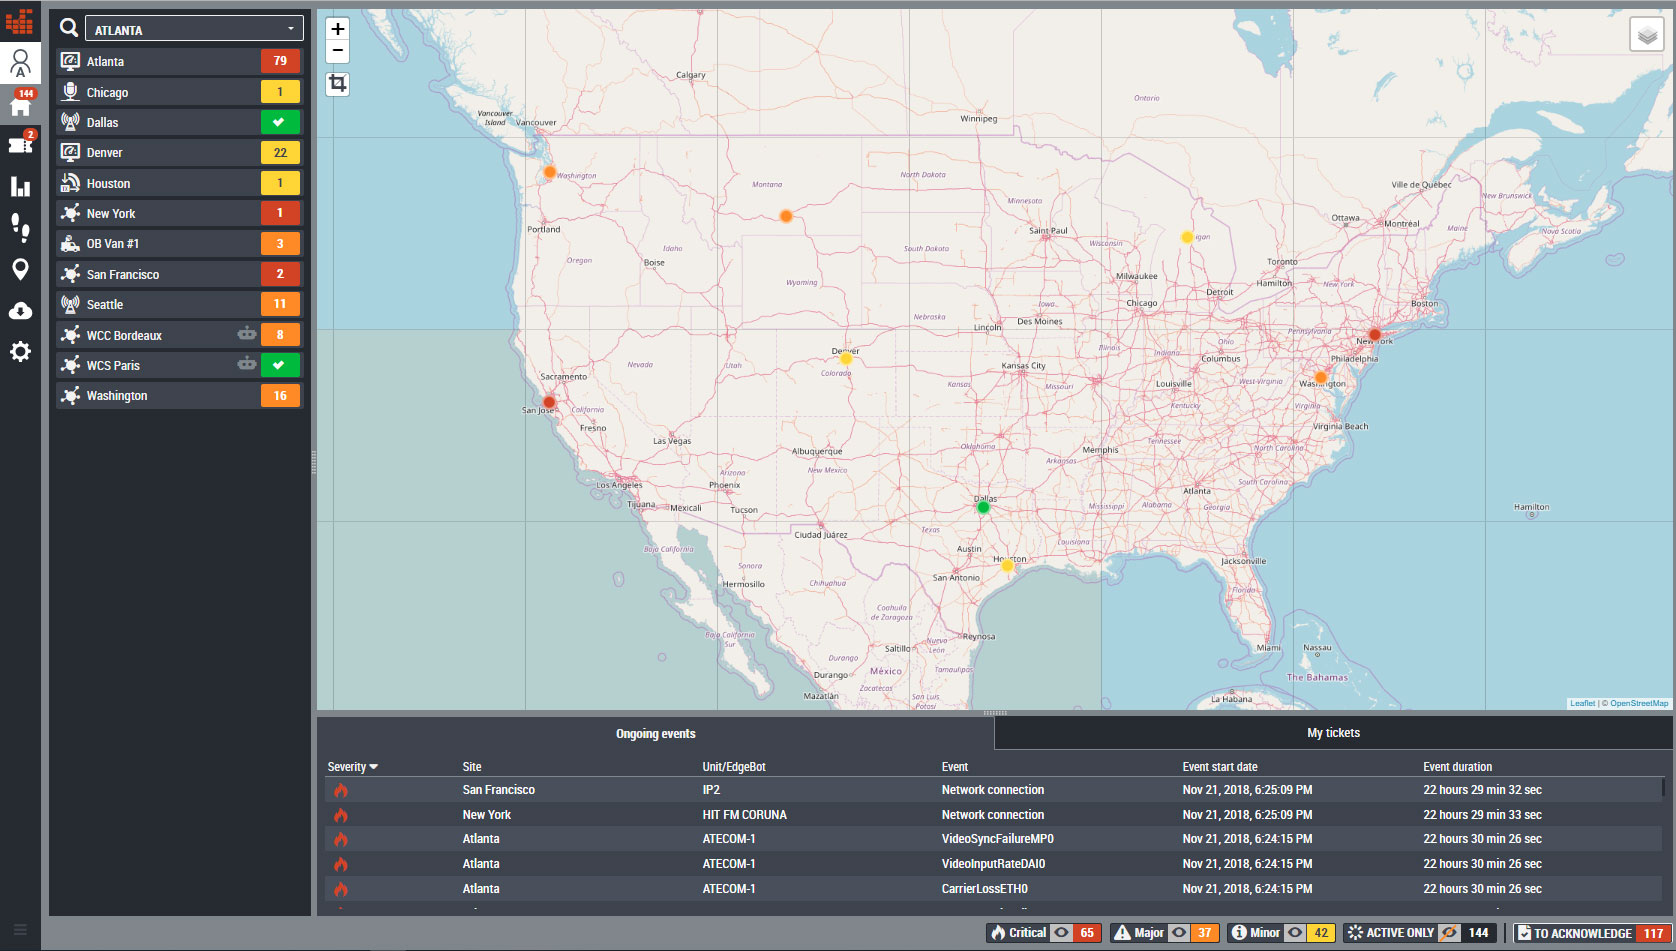
\includegraphics[width=0.8\textwidth]{fig/research/worldcast/dashboard.jpg}}
      \only<+>{\vspace*{-0.5cm}\includegraphics[width=0.8\textwidth]{fig/research/worldcast/readings.jpg}}
    \end{figure}

  \end{minipage}
  \begin{figure}[htp]
    \centering
    \includegraphics[width=\textwidth]{fig/frise20}
  \end{figure}
\end{frame}

\begin{frame}[t]{Axe de recherche 2 : IA pour la construction de codes}
  \begin{minipage}[t][5.0cm][t]{\textwidth}
    \begin{columns}[T]
      \begin{column}{0.45\textwidth}
        \vspace*{-1.1cm}
        \begin{center}
          \only<+>{\includegraphics[width=\textwidth]{fig/research/ai_codes/schema_ai_coding_left_1}}
          \only<+->{\includegraphics[width=\textwidth]{fig/research/ai_codes/schema_ai_coding_left_2}}
        \end{center}
      
        \vspace*{-1cm}
        \small{
        \begin{itemize}
          \setlength\itemsep{-0.5em}
          \item[\GREEN{$+$}]<9-> \GREEN{reproductible}
          \item[\GREEN{$+$}]<10-> \GREEN{faible complexité}
          \item[\RED{$-$}]  <11-> \RED  {a priori : SC}
          \item[\RED{$-$}]  <11-> \RED  {a priori : AWGN}
          % \item[\RED{$-$}]  <+-> \RED  {non optimal}
          \item[\RED{$-$}]  <11-> \RED  {spécifique au code}
        \end{itemize}
        }
      \end{column}
      \begin{column}{0.04\textwidth}
      \end{column}
      \begin{column}{0.45\textwidth}
        \vspace*{-1.1cm}
        \begin{center}
          \only<+>{\includegraphics[width=\textwidth]{fig/research/ai_codes/schema_ai_coding_right_1}}
          \only<+>{\includegraphics[width=\textwidth]{fig/research/ai_codes/schema_ai_coding_right_2}}
          \only<+>{\includegraphics[width=\textwidth]{fig/research/ai_codes/schema_ai_coding_right_3}}
          \only<+>{\includegraphics[width=\textwidth]{fig/research/ai_codes/schema_ai_coding_right_4}}
          \only<+>{\includegraphics[width=\textwidth]{fig/research/ai_codes/schema_ai_coding_right_5}}
          \only<+->{\includegraphics[width=\textwidth]{fig/research/ai_codes/schema_ai_coding_right_6}}
        \end{center}
        \vspace*{-1cm}
        \small{
        \begin{itemize}
          \setlength\itemsep{-0.5em}
          \item[\RED{$-$}]  <+-> \RED  {non reproductible}
          \item[\RED{$-$}]  <+-> \RED  {forte complexité}
          \item[\GREEN{$+$}]<+-> \GREEN{s'adapte au décodeur}
          \item[\GREEN{$+$}]<11> \GREEN{s'adapte au canal}
          \item[\GREEN{$+$}]<11> \GREEN{méthode générique}
        \end{itemize}
        }
      \end{column}
    \end{columns}
      \only<3>
        {
          \vspace*{-2.5cm}
          \renewcommand{\section}[2]{} % Trick to avoid references section
          \renewcommand*{\bibfont}{\scriptsize}
          \nocite{ai_coding}
          \printbibliography[keyword={ai_coding}]
        }
  \end{minipage}
  \begin{figure}[htp]
    \centering
    \includegraphics[width=\textwidth]{fig/frise24}
  \end{figure}
\end{frame}


\begin{frame}[t]{Axe de recherche 2 : IA pour la construction de codes}
  \begin{minipage}[t][5.0cm][t]{\textwidth}
    \begin{center}
      Un simulateur performant \& générique : AFF3CT
    \end{center}
    \begin{itemize}
      \item[\RED{$-$}]  <+-> \RED  {forte complexité} $\rightarrow$ simulateur performant
      \item[\GREEN{$+$}]<+-> \GREEN{méthode générique} $\rightarrow$ nombreux codes
      \item[\GREEN{$+$}]<+-> \GREEN{s'adapte au décodeur} $\rightarrow$ nombreux algorithmes
      \item[\GREEN{$+$}]<+-> \GREEN{s'adapte au canal} $\rightarrow$ nombreux modèles de canal
      \item[\GREEN{$+$}]<+-> \GREEN{s'adapte à l'implémentation} $\rightarrow$ décodeurs génériques et flexibles
    \end{itemize}
\end{minipage}
\begin{figure}[htp]
  \centering
  \includegraphics[width=\textwidth]{fig/frise24}
\end{figure}
\end{frame}


\begin{frame}[t]{International collaborations}
  \begin{minipage}[t][5.0cm][t]{\textwidth}
      \vspace{-0.4cm}
    \begin{columns}[T]
      \begin{column}{0.63\textwidth}
        \small{
          \begin{itemize}
            \item<+-> Co-supervised thesis between University of Bordeaux and Polytechnique Montréal (Canada)
            \begin{itemize}
            \item<1-> Yvon Savaria, director
            \item<1-> Pierre Langlois, co-author
            \begin{itemize}
              \item<+->[$\rightarrow$] Architecture-Algorithm Adequation
            \end{itemize}
            \end{itemize}
            \vspace{0.25cm}
            \item<+-> Thibaud Tonnellier, McGill University (Canada), co-author
            \begin{itemize}
              \item<+->[$\rightarrow$] Polar Codes \& AI
            \end{itemize}
          \end{itemize}
        }
      \end{column}
      \begin{column}{0.04\textwidth}
      \end{column}
      \begin{column}{0.33\textwidth}
      \centering
        \only<1->{\vspace{0.8cm}\includegraphics[width=0.5\textwidth]{fig/poly}\\\vspace{1.6cm} }
        \only<3->{\includegraphics[width=0.5\textwidth]{fig/mcgill}\\}
      \end{column}
    \end{columns}
  \end{minipage}
  \begin{figure}[htp]
    \centering
    \includegraphics[width=\textwidth]{fig/frise23}
  \end{figure}
\end{frame}


\begin{frame}[t]{International collaborations}
  \begin{minipage}[t][5.0cm][t]{\textwidth}
      \vspace{-0.3cm}
    \begin{columns}[T]
      \begin{column}{0.63\textwidth}
        \small{
          \begin{itemize}
            \item<+-> Pekka Jääskelainen, TUT (Finland), co-author
            \begin{itemize}
              \item<+->[$\rightarrow$] ASIP
            \end{itemize}
            \item<+-> Vyacheslav Klymentiev, Saint Petersburg Electrotechnical University (Russia)
            \item<3-> Peter Trifonov, Saint Petersburg Polytechnic University (Russia)
            \item<3-> Chen Shuang, Tsinghua University (China)
            \begin{itemize}
              \item<+->[$\rightarrow$] AFF3CT
            \end{itemize}
          \end{itemize}
        }
      \end{column}
      \begin{column}{0.04\textwidth}
      \end{column}
      \begin{column}{0.33\textwidth}
      \centering
        \only<1->{\includegraphics[width=1\textwidth]{fig/tampere}\\\vspace{-0.1cm}}
        \only<3->{\includegraphics[width=0.26\textwidth]{fig/etu}\\\vspace{0.5cm}}
        \only<3->{\includegraphics[width=0.5\textwidth]{fig/polysp}\vspace{-0.2cm}\\}
        \only<3->{\includegraphics[width=0.7\textwidth]{fig/tsinghua}}

      \end{column}
    \end{columns}
  \end{minipage}
  \begin{figure}[htp]
    \centering
    \includegraphics[width=\textwidth]{fig/frise23}
  \end{figure}
\end{frame}


\begin{frame}[c]{}
\vfill
\centering
Merci pour votre attention !
\vfill
\end{frame}

\begin{frame}[c, noframenumbering]{ASIP : Compromis Flexibilité performance. }
  \begin{itemize}
    \item Une solution générique et pérenne de génération de DNN basse consommation,
    \item dimensionnement flexible : nombre de modules, interconnexion, multic\oe{}urs,
    \item évolutions après fabrication (programmabilité),
    \item pour l'équipe de recherche : capitalisation.
  \end{itemize}
  \centering
  \includegraphics[width=0.6\textwidth]{fig/tta_base}
\end{frame}

\begin{frame}[t, noframenumbering]{Plateformes hétérogènes pour l'IA}
  \begin{minipage}[t][5.0cm][t]{\textwidth}
    \vspace{-0.5cm}
    \begin{itemize}
      \item<+-> De nombreuses plateformes potentielles (CPU, GPU, FPGA, TPU)
      \item<+-> ... et leurs combinaisons (architectures hétérogènes).
      \item<+-> Il est nécessaire d'en réaliser l'abstraction
      \begin{itemize}
        \item<+-> des bibliothèques logicielles pour calcul parallèle (C++ STL, SyCL),
        \item<+-> des langages et compilateurs pour cibles parallèles (OpenCL, TCE),
        \item<+-> des langages (SystemC, System Verilog) et outils de synthèse matérielle haut niveau (Vivado HLS,
        Intel HLS Compiler)
      \end{itemize}
    \end{itemize}
  \end{minipage}

\end{frame}

\begin{frame}[t, noframenumbering]{IA pour la construction de codes}
  \centering
  \includegraphics[width=\textwidth]{fig/research/ai_codes/schema_ai_coding_right_6}
\end{frame}

\end{document}


% \begin{frame}[t]{Axe de recherche 1 : Codes Polaires}
%   \begin{minipage}[t][5.0cm][t]{\textwidth}
%     \begin{columns}[T]
%       \begin{column}{0.63\textwidth}
%         \vspace{-0.5cm}
%         \begin{itemize}
%           \item<+-> Expertise développée au cours de ma thèse
%           \item<+-> Thèmes de recherche
%           \begin{itemize}
%             \item<+-> Implémentations matérielles flexibles
%             \item<+-> Implémentations logicielles hautes performance
%             \item<+-> Algorithmes à sortie souple
%             \item<+-> Nouvelles constructions : multinoyaux, assymétriques
%           \end{itemize}
%         \end{itemize}
%       \end{column}
%       \begin{column}{0.04\textwidth}

%       \end{column}
%       \begin{column}{0.33\textwidth}
%         \only<1->{\includegraphics[width=\textwidth]{fig/sc}\\ \vspace{0.5cm}}
%         \only<3->{\includegraphics[width=\textwidth]{fig/ilp-1}}
%       \end{column}
%     \end{columns}
%   \end{minipage}
%   \begin{figure}[htp]
%     \centering
%     \includegraphics[width=\textwidth]{fig/frise20}
%   \end{figure}
% \end{frame}

% \begin{frame}[t]{Axe de recherche 2 : Adéquation algorithme - architecture}
%   \begin{minipage}[t][5.0cm][t]{\textwidth}
%     \begin{columns}[T]
%       \begin{column}{0.48\textwidth}
%         \begin{itemize}
%           \item<+-> Modulation (FBMC/OQAM)
%           \item<+-> Entrelaceurs de turbo-codes
%           \item<+-> Modulation codée
%           \item<+-> ...
%           \vspace{0.5cm}
%           \item<+-> Implémentations logicielles
%           \item<+-> Implémentations matérielles
%           \item<+-> Simplifications algorithmiques
%         \end{itemize}
%       \end{column}
%       \begin{column}{0.04\textwidth}
%       \end{column}
%       \begin{column}{0.48\textwidth}
%         \begin{itemize}
%           \item<+-> Exemple : SCMA
%           \item<+-> Approximations calculatoires
%           \item<+-> Implémentation logicielle parallélisée
%           \item<+-> Débit augmenté de plusieurs ordres de grandeur
%         \end{itemize}
%         % \only<1->{\includegraphics[width=0.3\textwidth]{fig/aff3ct}\\ \vspace{0.2cm}}
%         % \only<2->{\includegraphics[width=\textwidth]{fig/usrp}}
%       \end{column}
%     \end{columns}
%   \end{minipage}
%   \begin{figure}[htp]
%     \centering
%     \includegraphics[width=\textwidth]{fig/frise21}
%   \end{figure}
% \end{frame}

% \begin{frame}[t]{Axe de recherche 3 : Architectures ASIP}
%   \begin{minipage}[t][5.0cm][t]{\textwidth}
%     \begin{itemize}
%       \item<+-> Nombreux travaux sur architectures ASIP (DecASIP)
%       \item<+-> Intégration : compétent sur les différents langages ASIP (incl. LISA + Synopsys)
%       \item<+-> Intégration : intérêt des architectures TTA
%     \end{itemize}
%     \only<1>{
%       \vspace{-2cm}
%       \begin{enumerate}
%         \renewcommand{\section}[2]{} % Trick to avoid references section
%         \renewcommand*{\bibfont}{\tiny}
%         \nocite{6579576,7155493,6654620,6683963,6571888,7041196}
%         \printbibliography[keyword={asip-amer}]
%       \end{enumerate}
%     }
%     \only<3>{
%       \centering
%       \includegraphics[width=0.6\textwidth]{fig/ilp-1}
%     }
%   \end{minipage}
%   \begin{figure}[htp]
%     \centering
%     \includegraphics[width=\textwidth]{fig/frise22}
%   \end{figure}
% \end{frame}